\documentclass[aspectratio=169]{beamer}

\usetheme{Madrid}
\usecolortheme{default}

\usepackage[utf8]{inputenc}
\usepackage[T1]{fontenc}
\usepackage[spanish]{babel}
\usepackage{amsmath}
\usepackage{booktabs}
\usepackage{graphicx}

\graphicspath{{Paper/figures/}{figures/}}
\newcommand{\tablepath}{Paper/tables/}
\setbeamertemplate{navigation symbols}{}
\setbeamertemplate{footline}[frame number]

\title{CJC Monitor}
\subtitle{Resultados preliminares}
\author{Centro Javeriano de Competitividad}
\date{\today}

\begin{document}

\begin{frame}
  \titlepage
\end{frame}

\begin{frame}{Motivacion}
  \begin{itemize}
    \item Escriba aqui la pregunta central del monitor.
    \item Resuma la contribucion principal.
  \end{itemize}
\end{frame}

\begin{frame}{Datos}
  \begin{itemize}
    \item Fuentes de datos.
    \item Periodo de analisis.
    \item Variables principales.
  \end{itemize}
\end{frame}

\begin{frame}{Establecimientos}
  \centering
  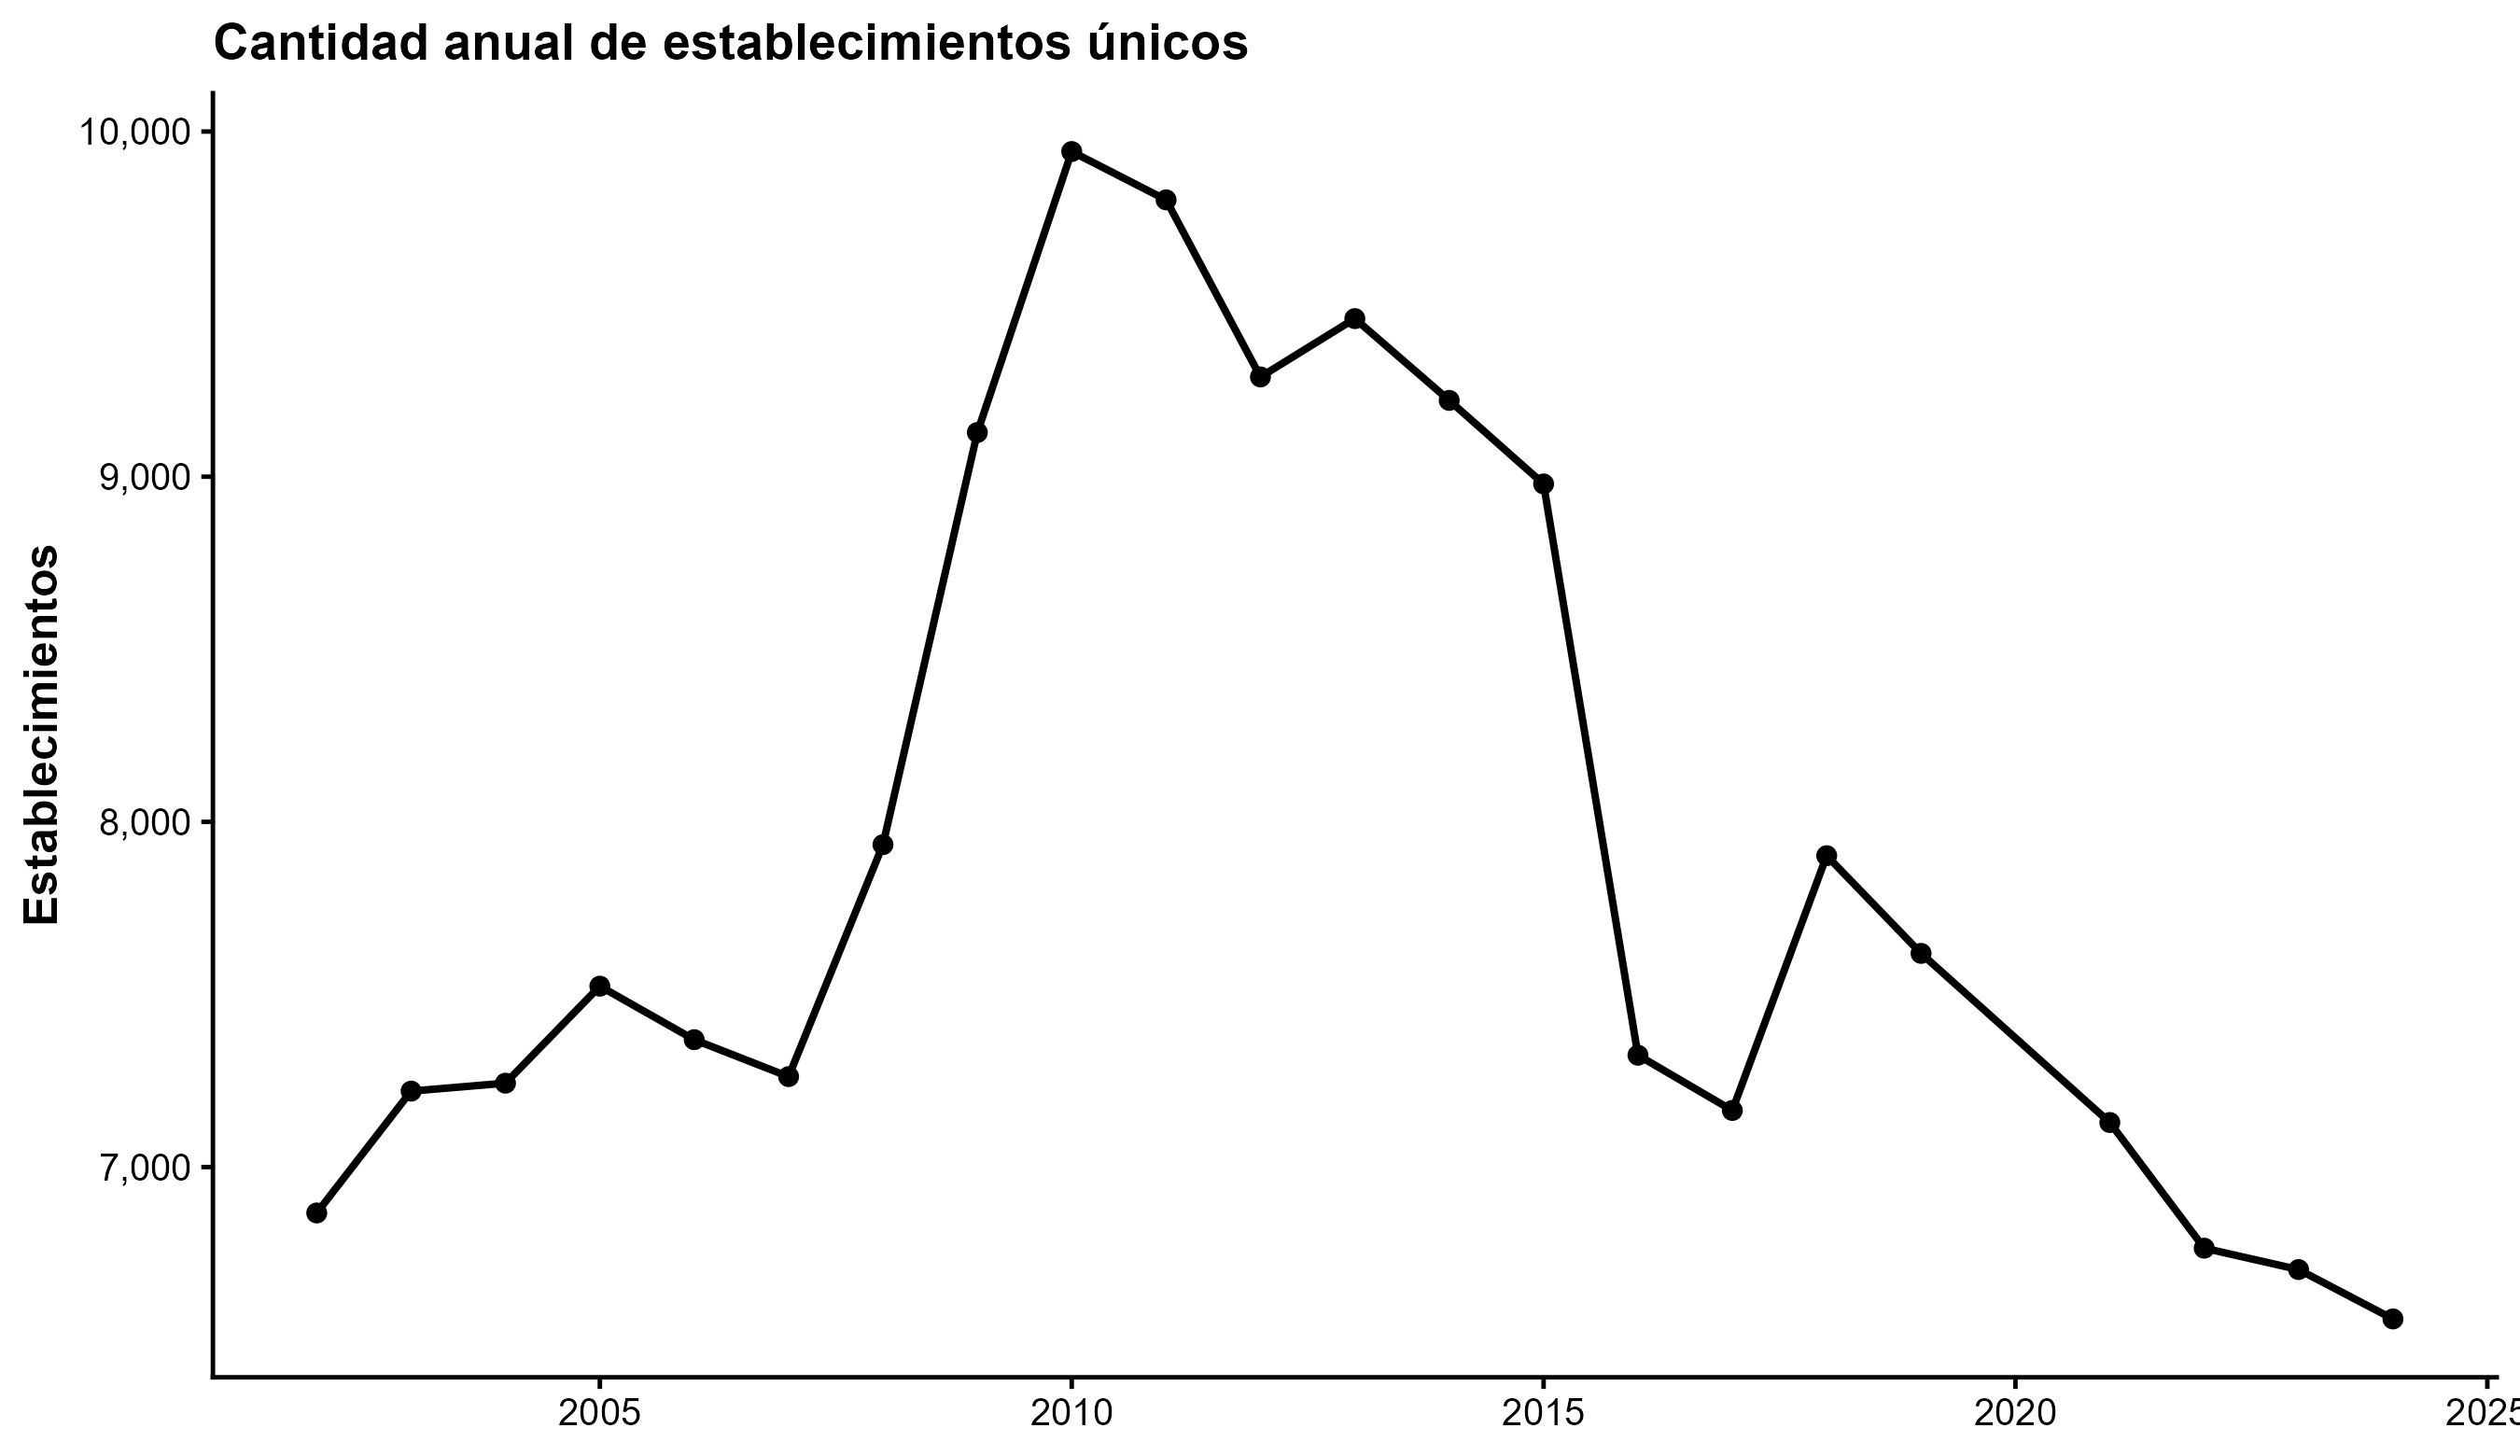
\includegraphics[width=0.9\linewidth]{fig1.png}
\end{frame}

\begin{frame}{Establecimientos por sector}
  \centering
  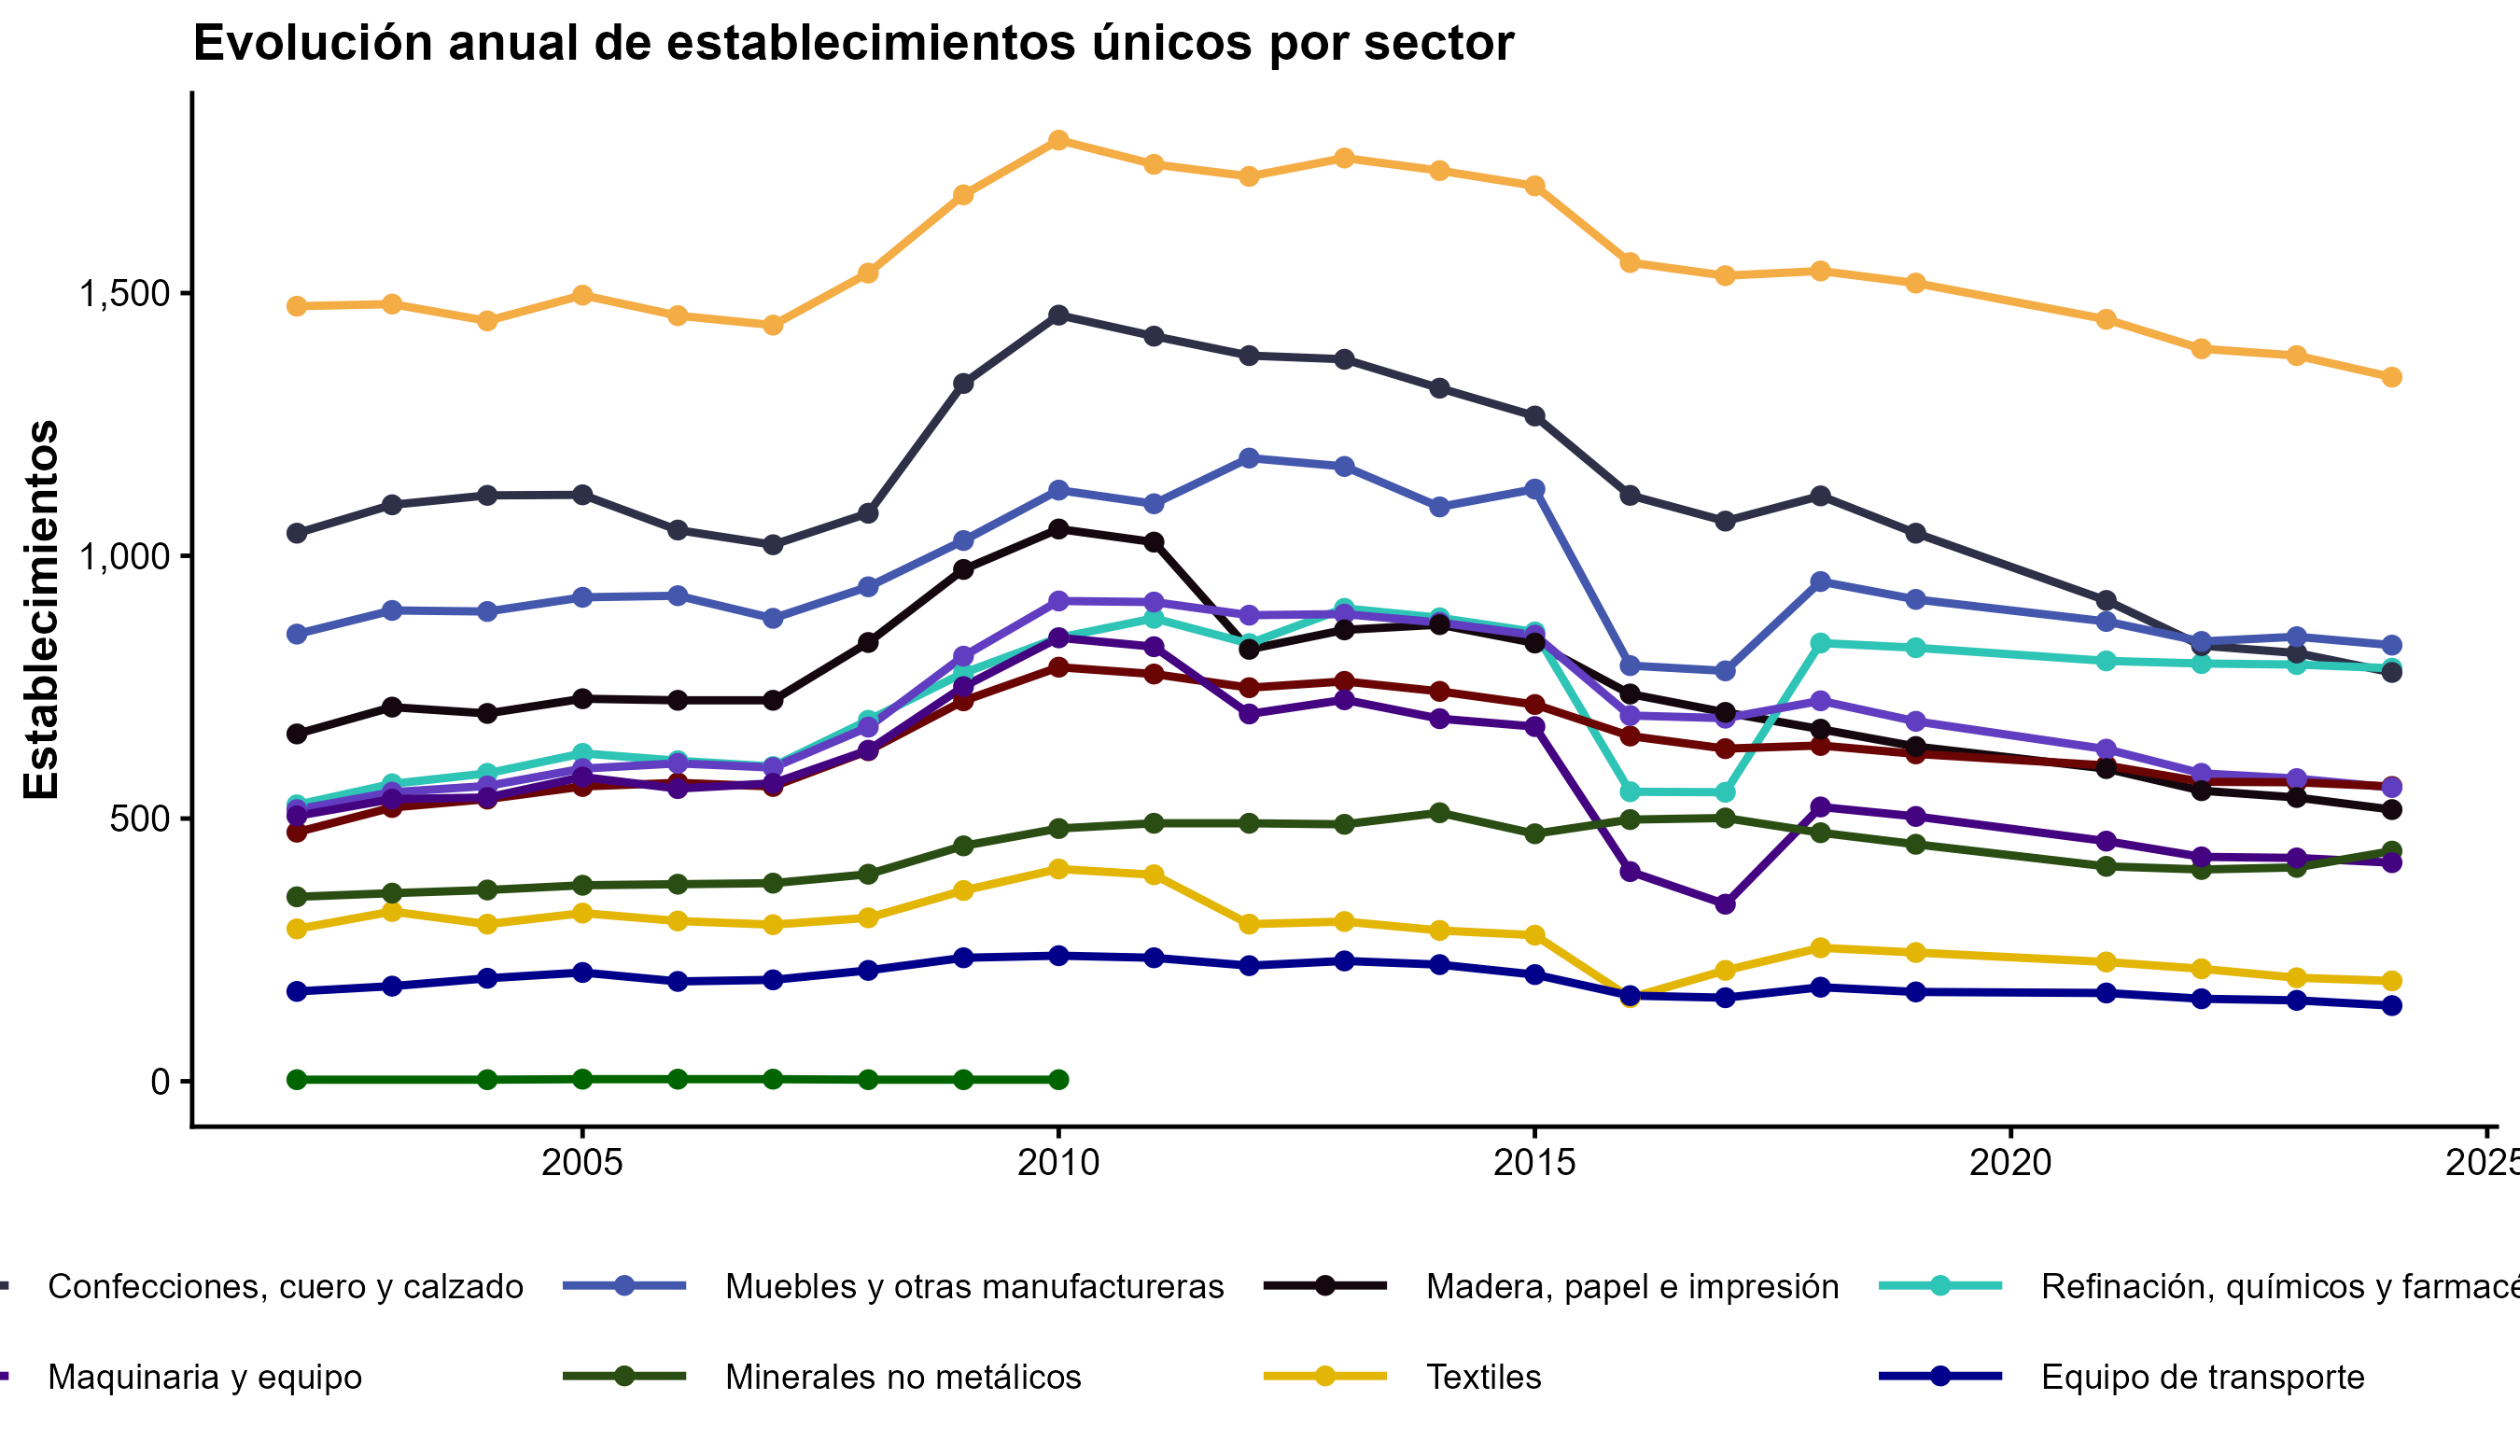
\includegraphics[width=0.9\linewidth]{fig2.png}
\end{frame}

\begin{frame}{Participacion por sector}
  \centering
  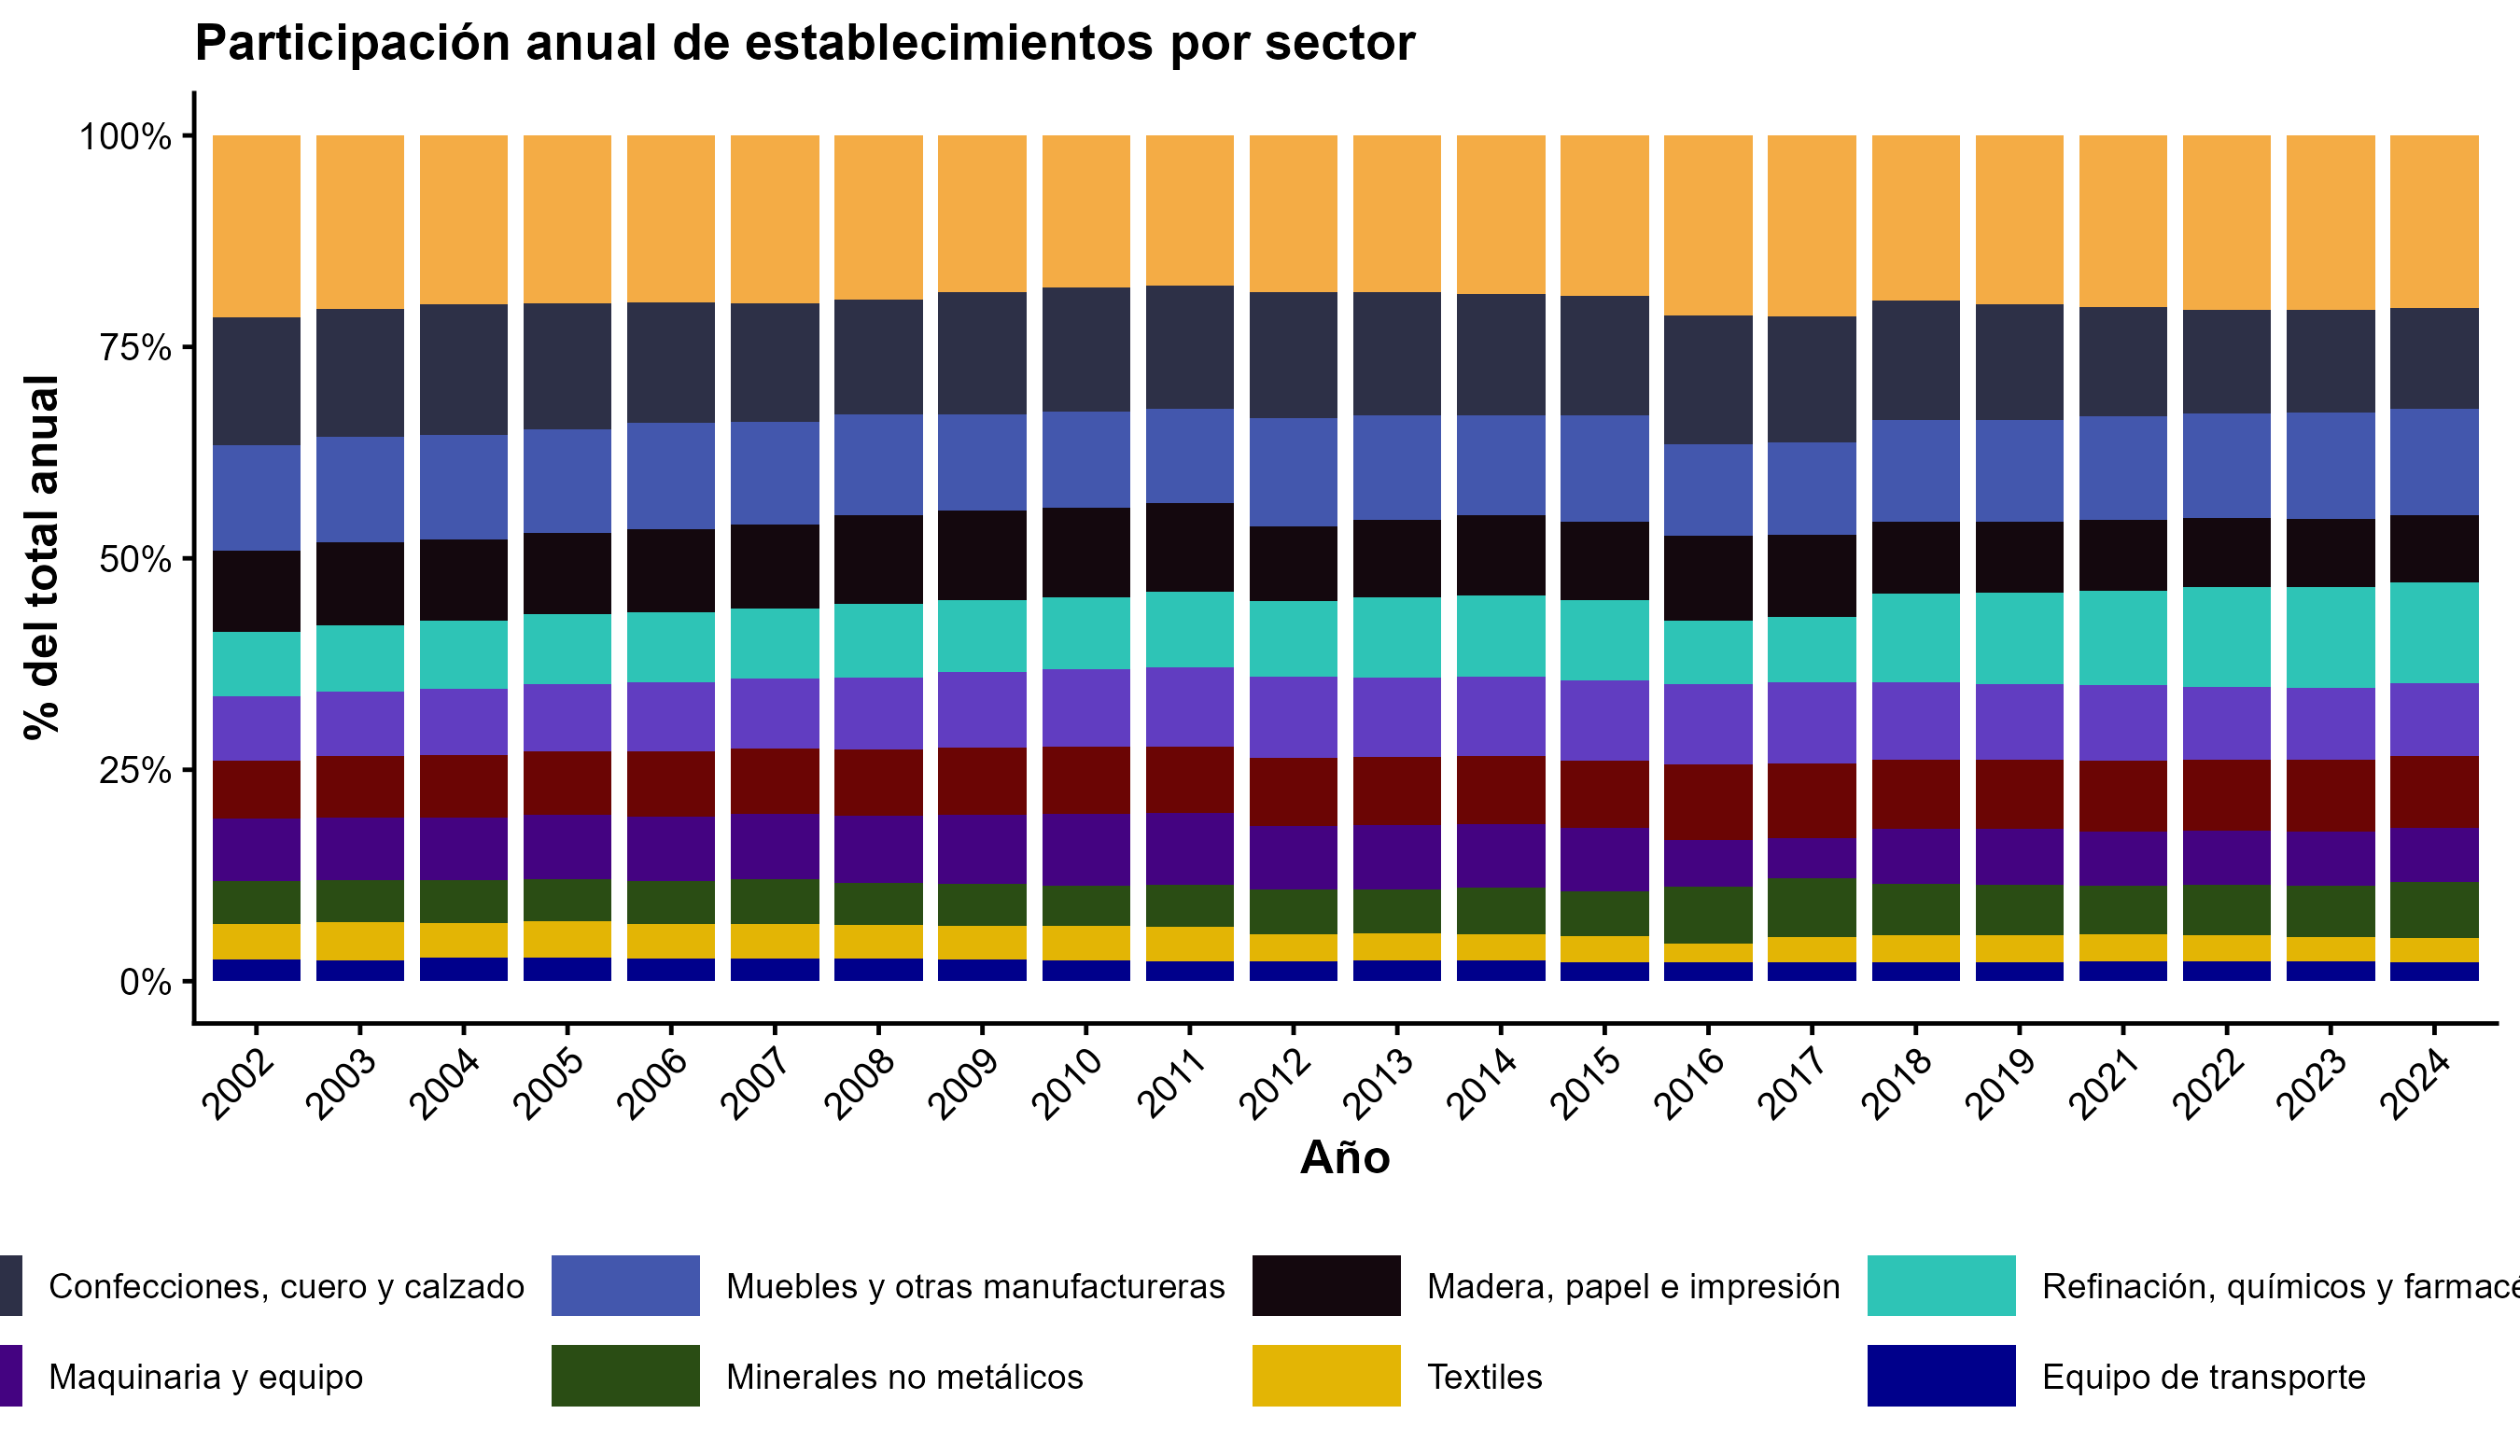
\includegraphics[width=0.9\linewidth]{fig3.png}
\end{frame}

\begin{frame}{Valor agregado por sector}
  \centering
  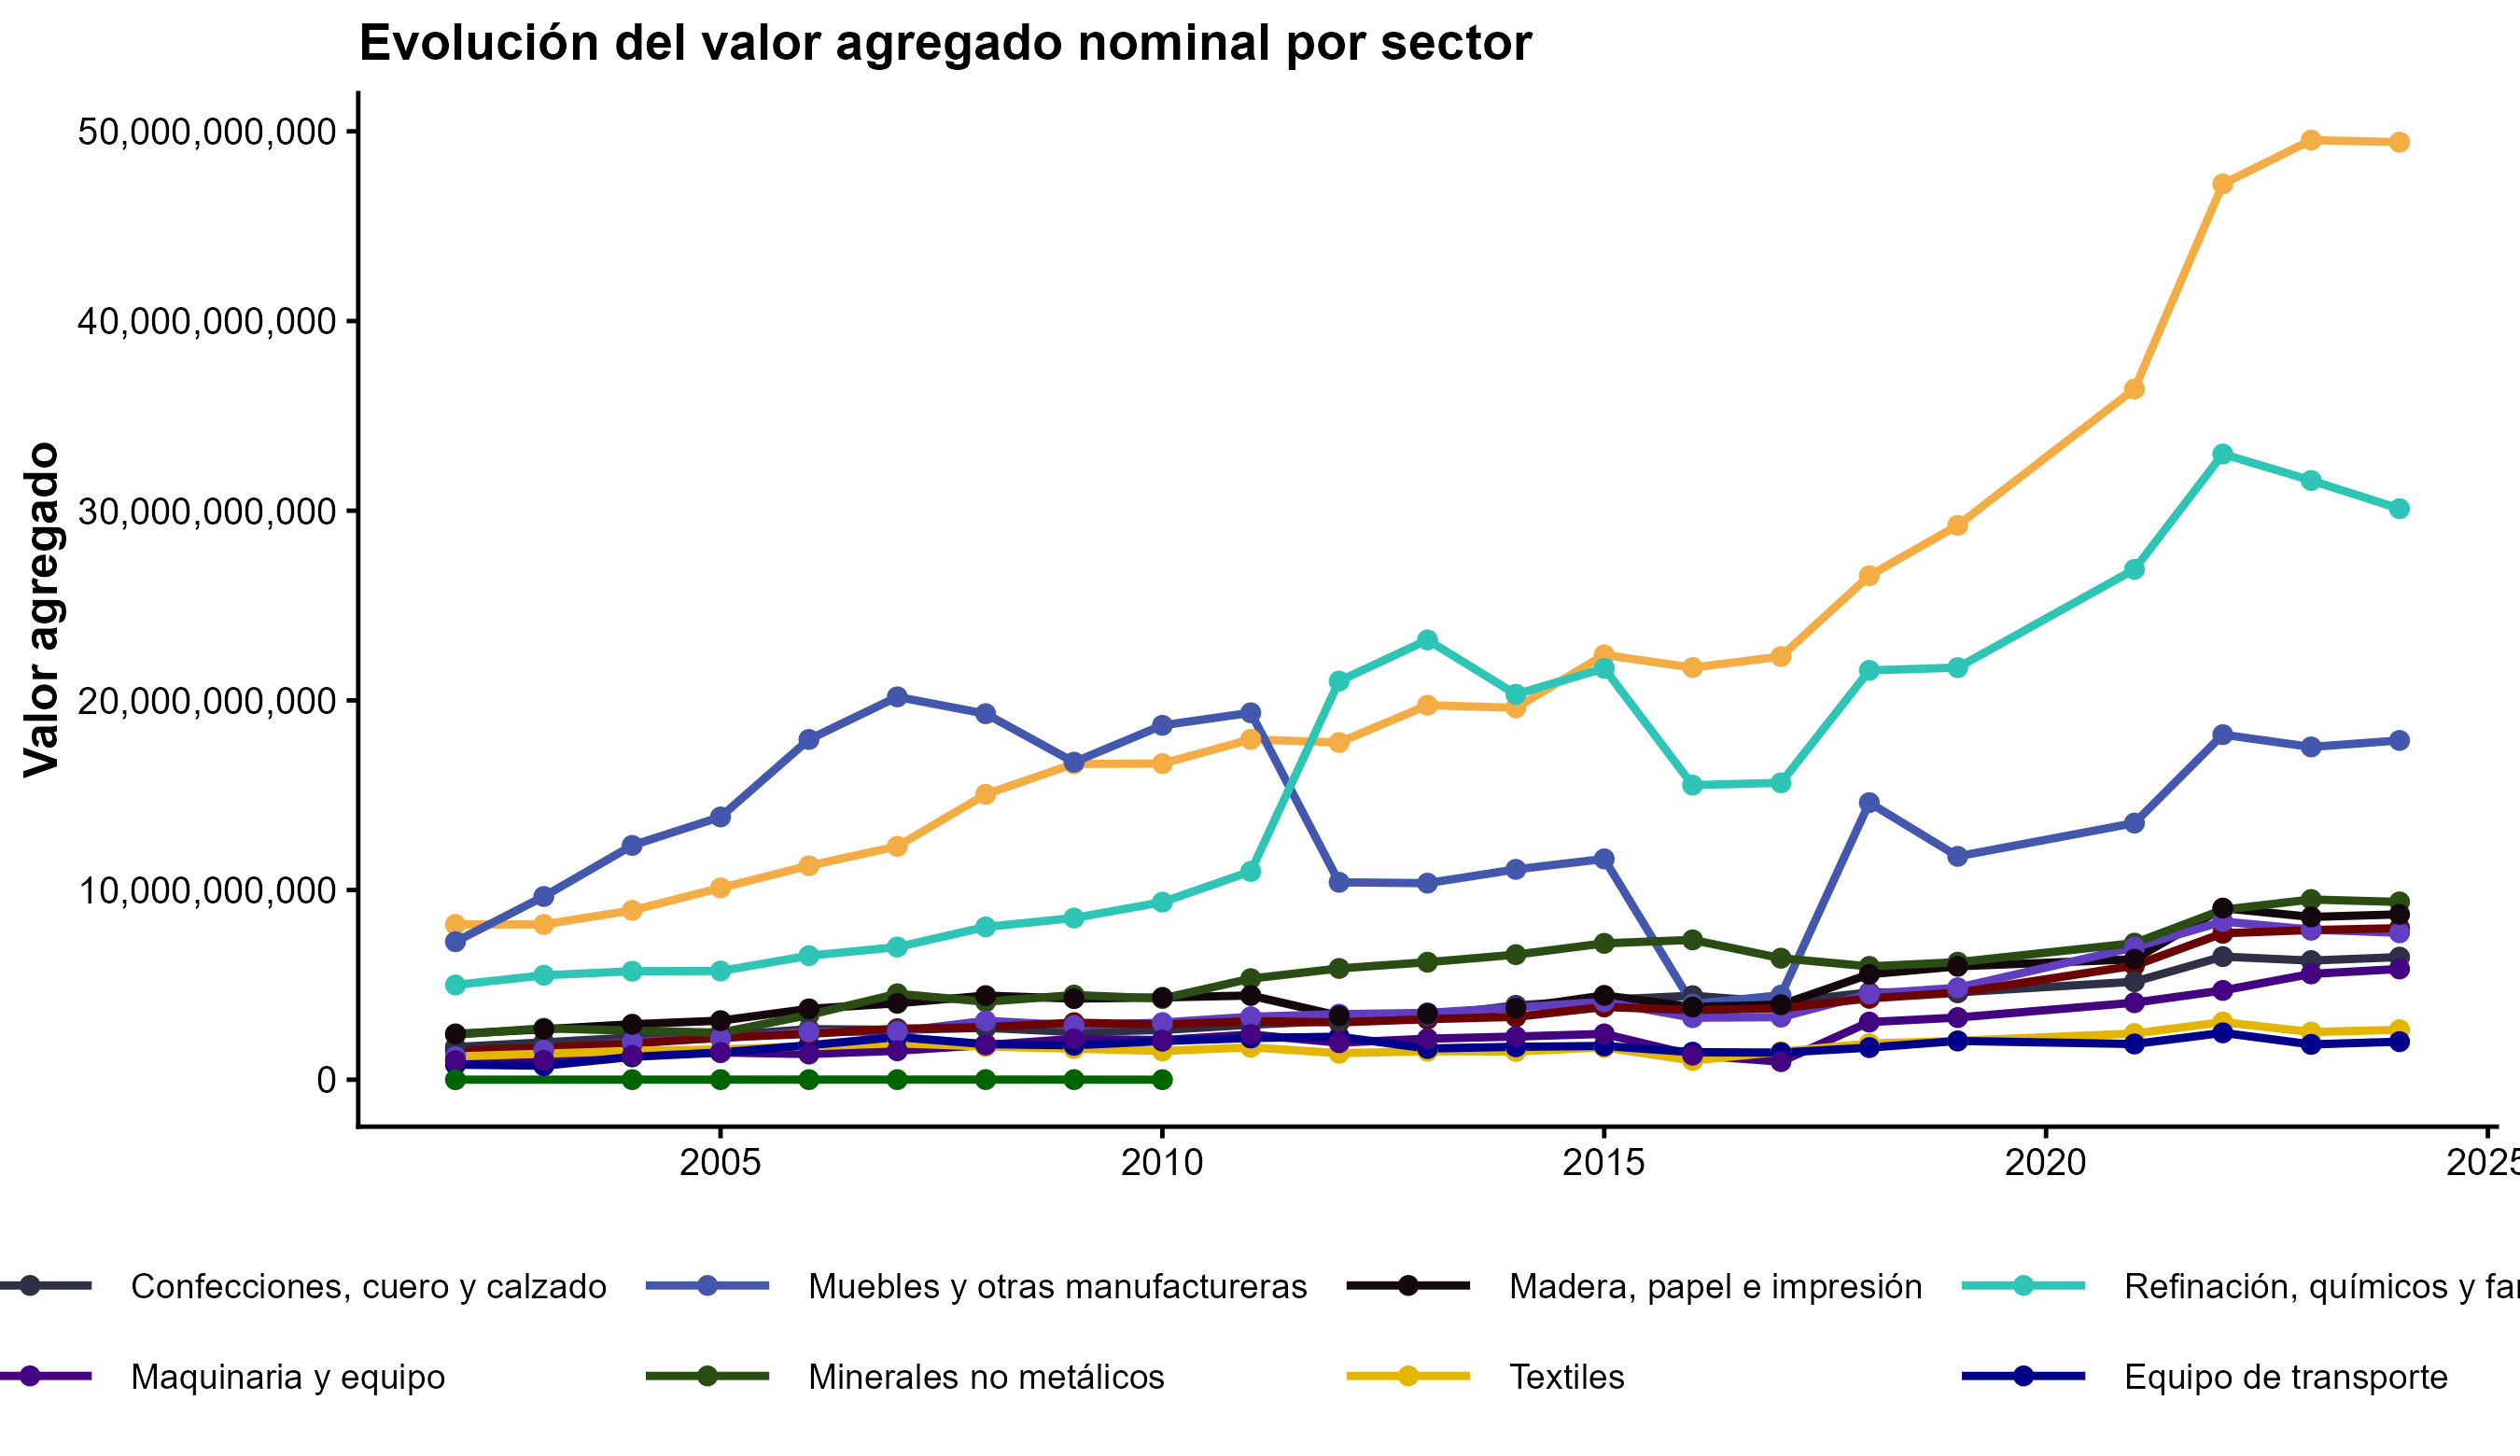
\includegraphics[width=0.9\linewidth]{fig4.png}
\end{frame}

\begin{frame}{Personal ocupado por sector}
  \centering
  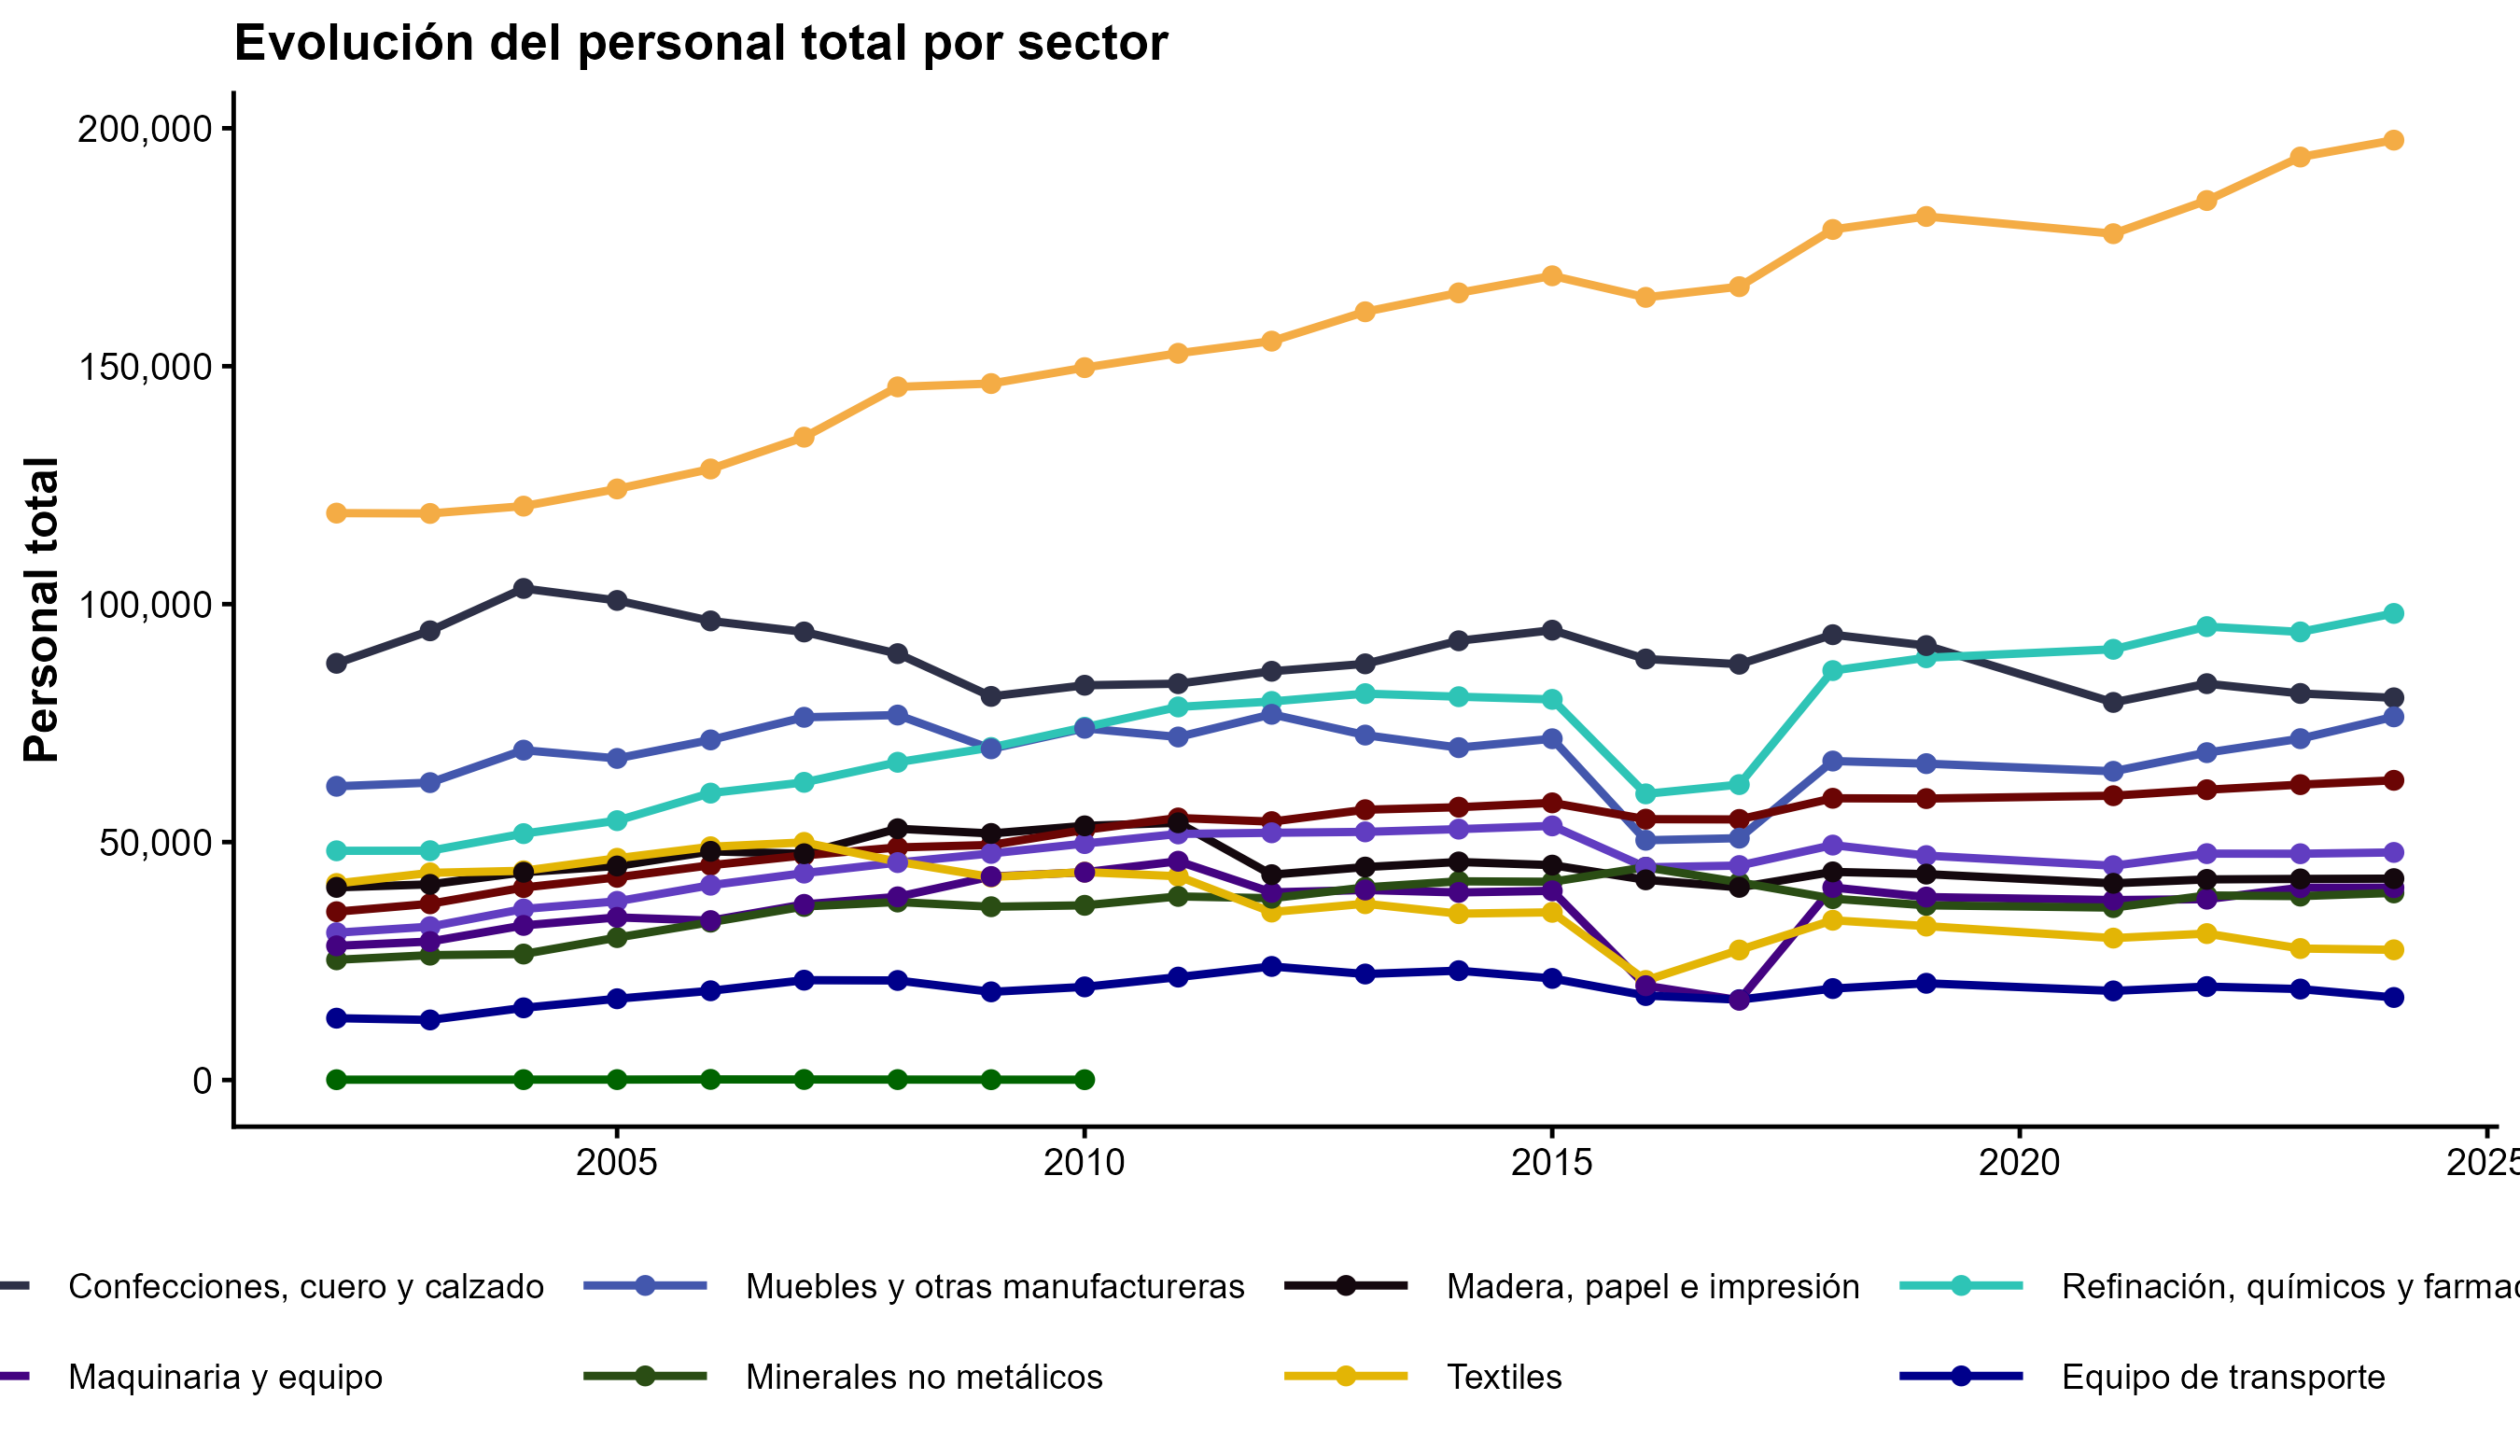
\includegraphics[width=0.9\linewidth]{fig5.png}
\end{frame}

\begin{frame}{Productividad por sector}
  \centering
  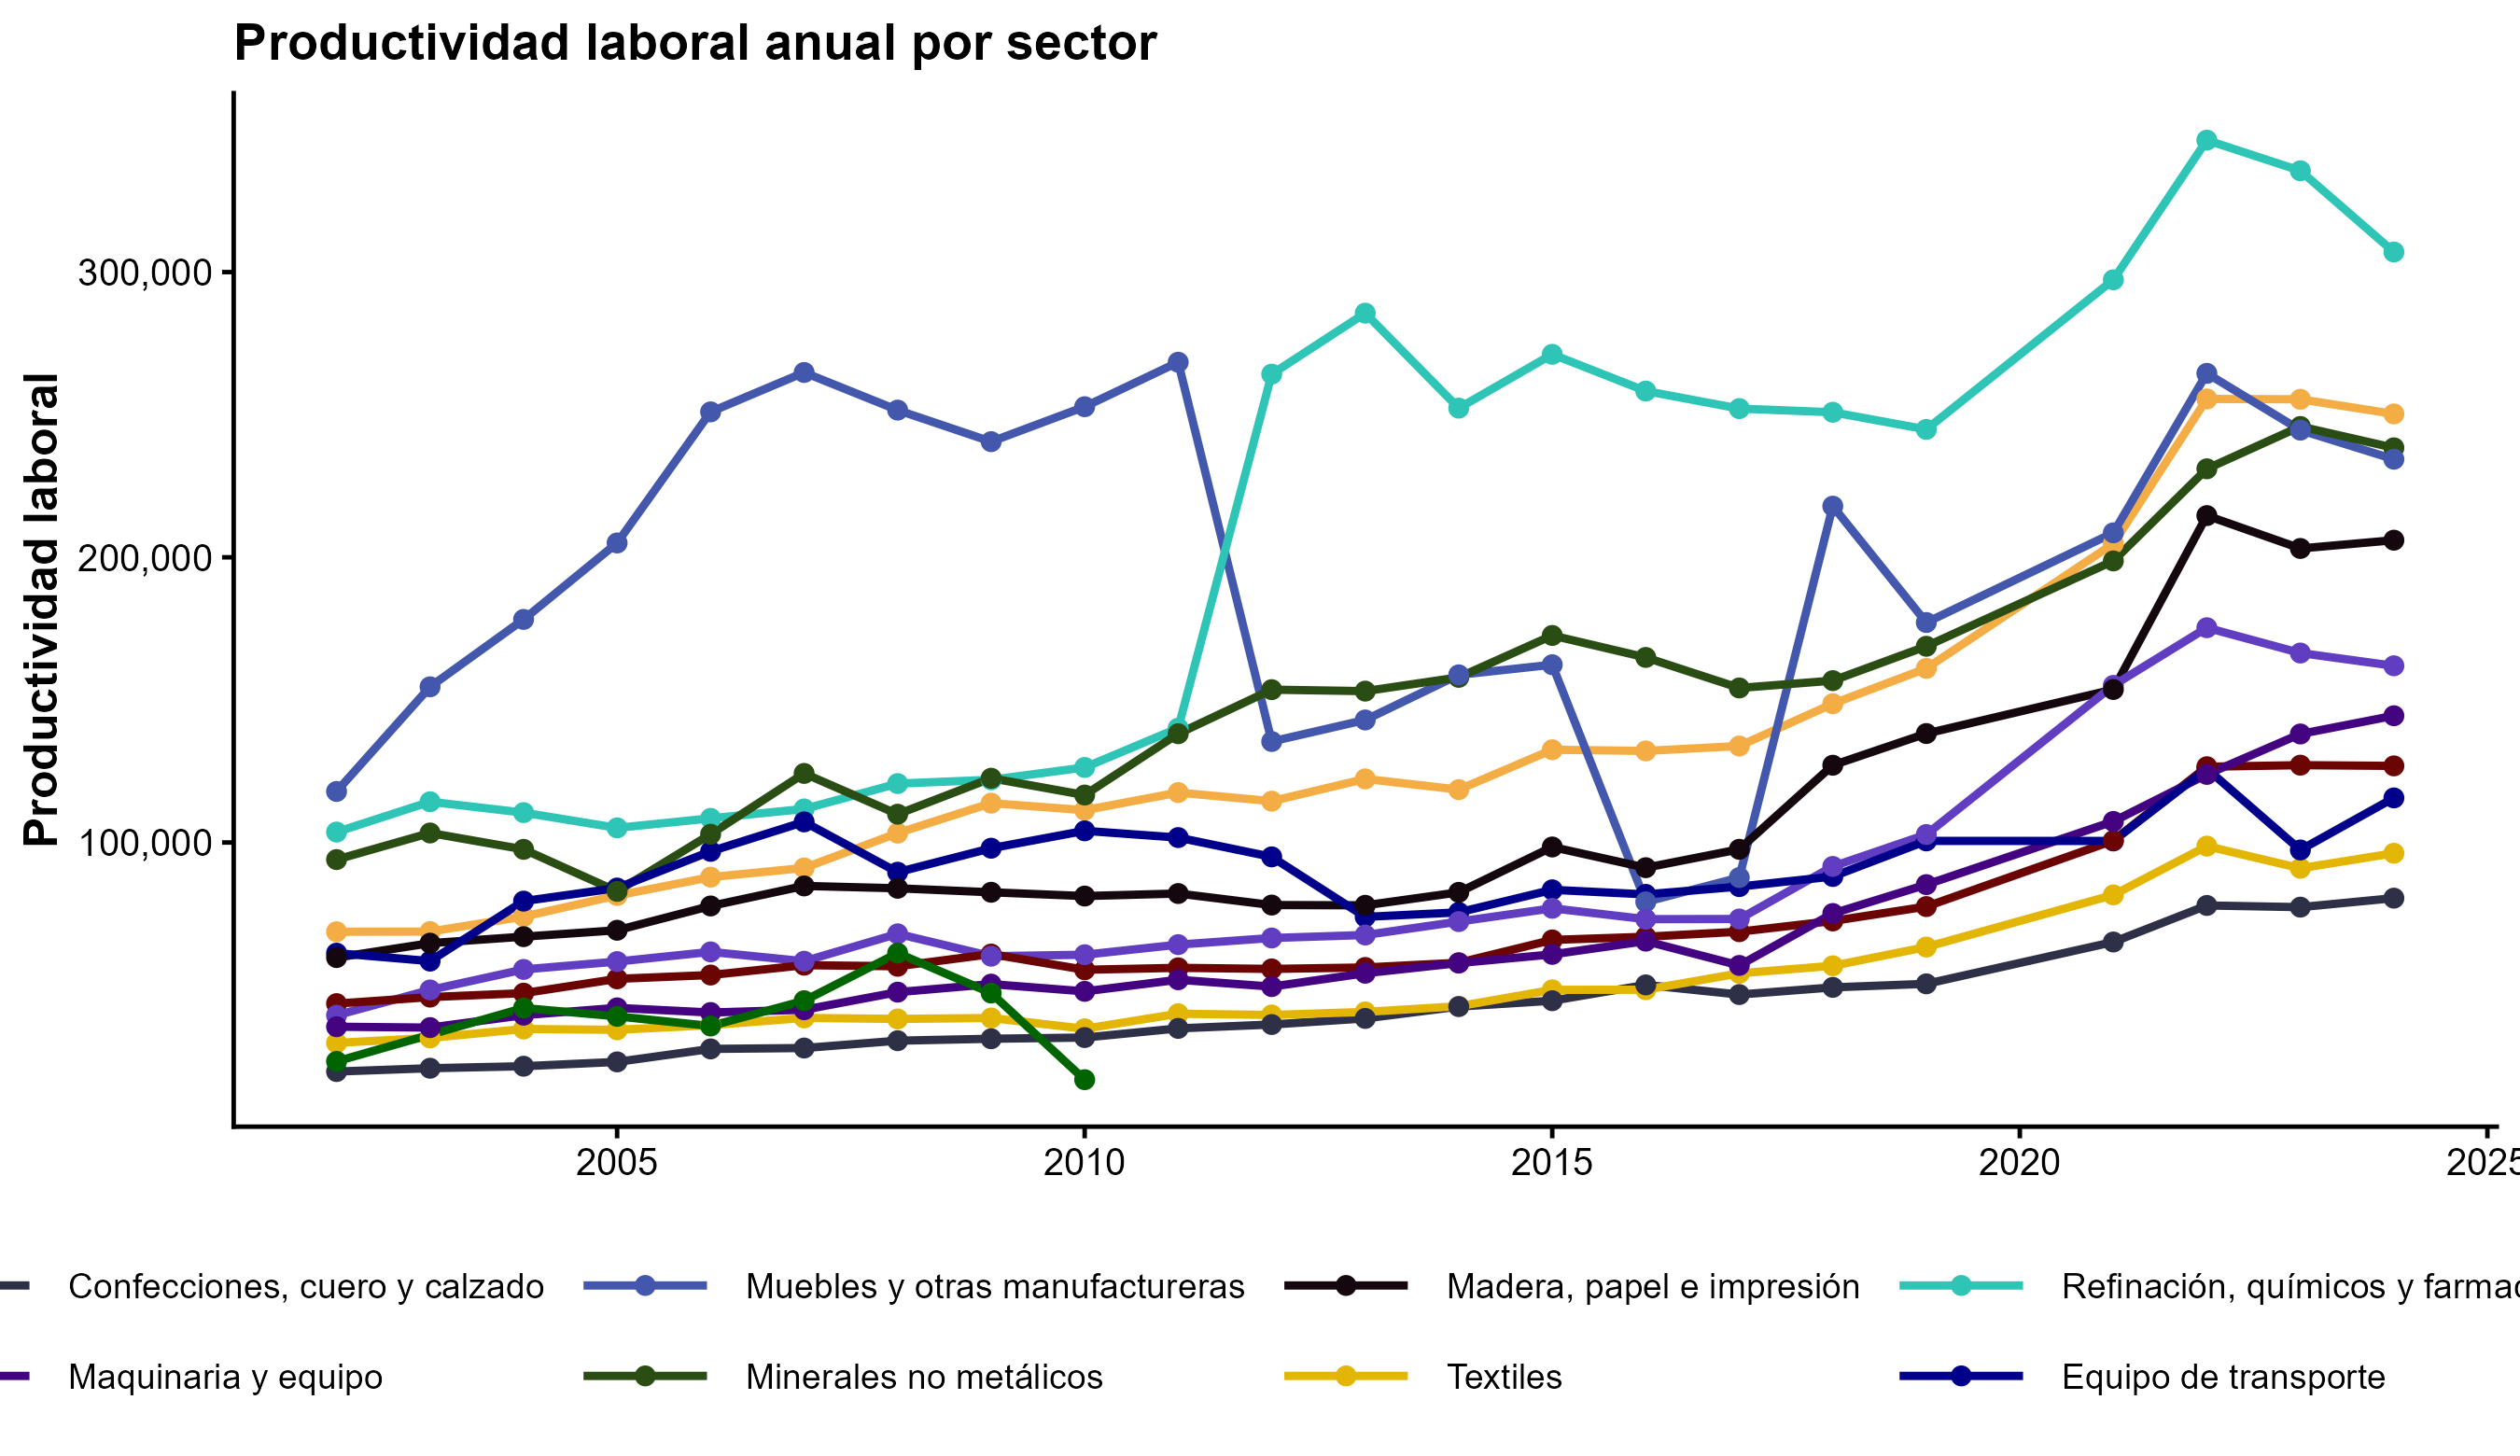
\includegraphics[width=0.9\linewidth]{fig6.png}
\end{frame}

\begin{frame}{Establecimientos por region}
  \centering
  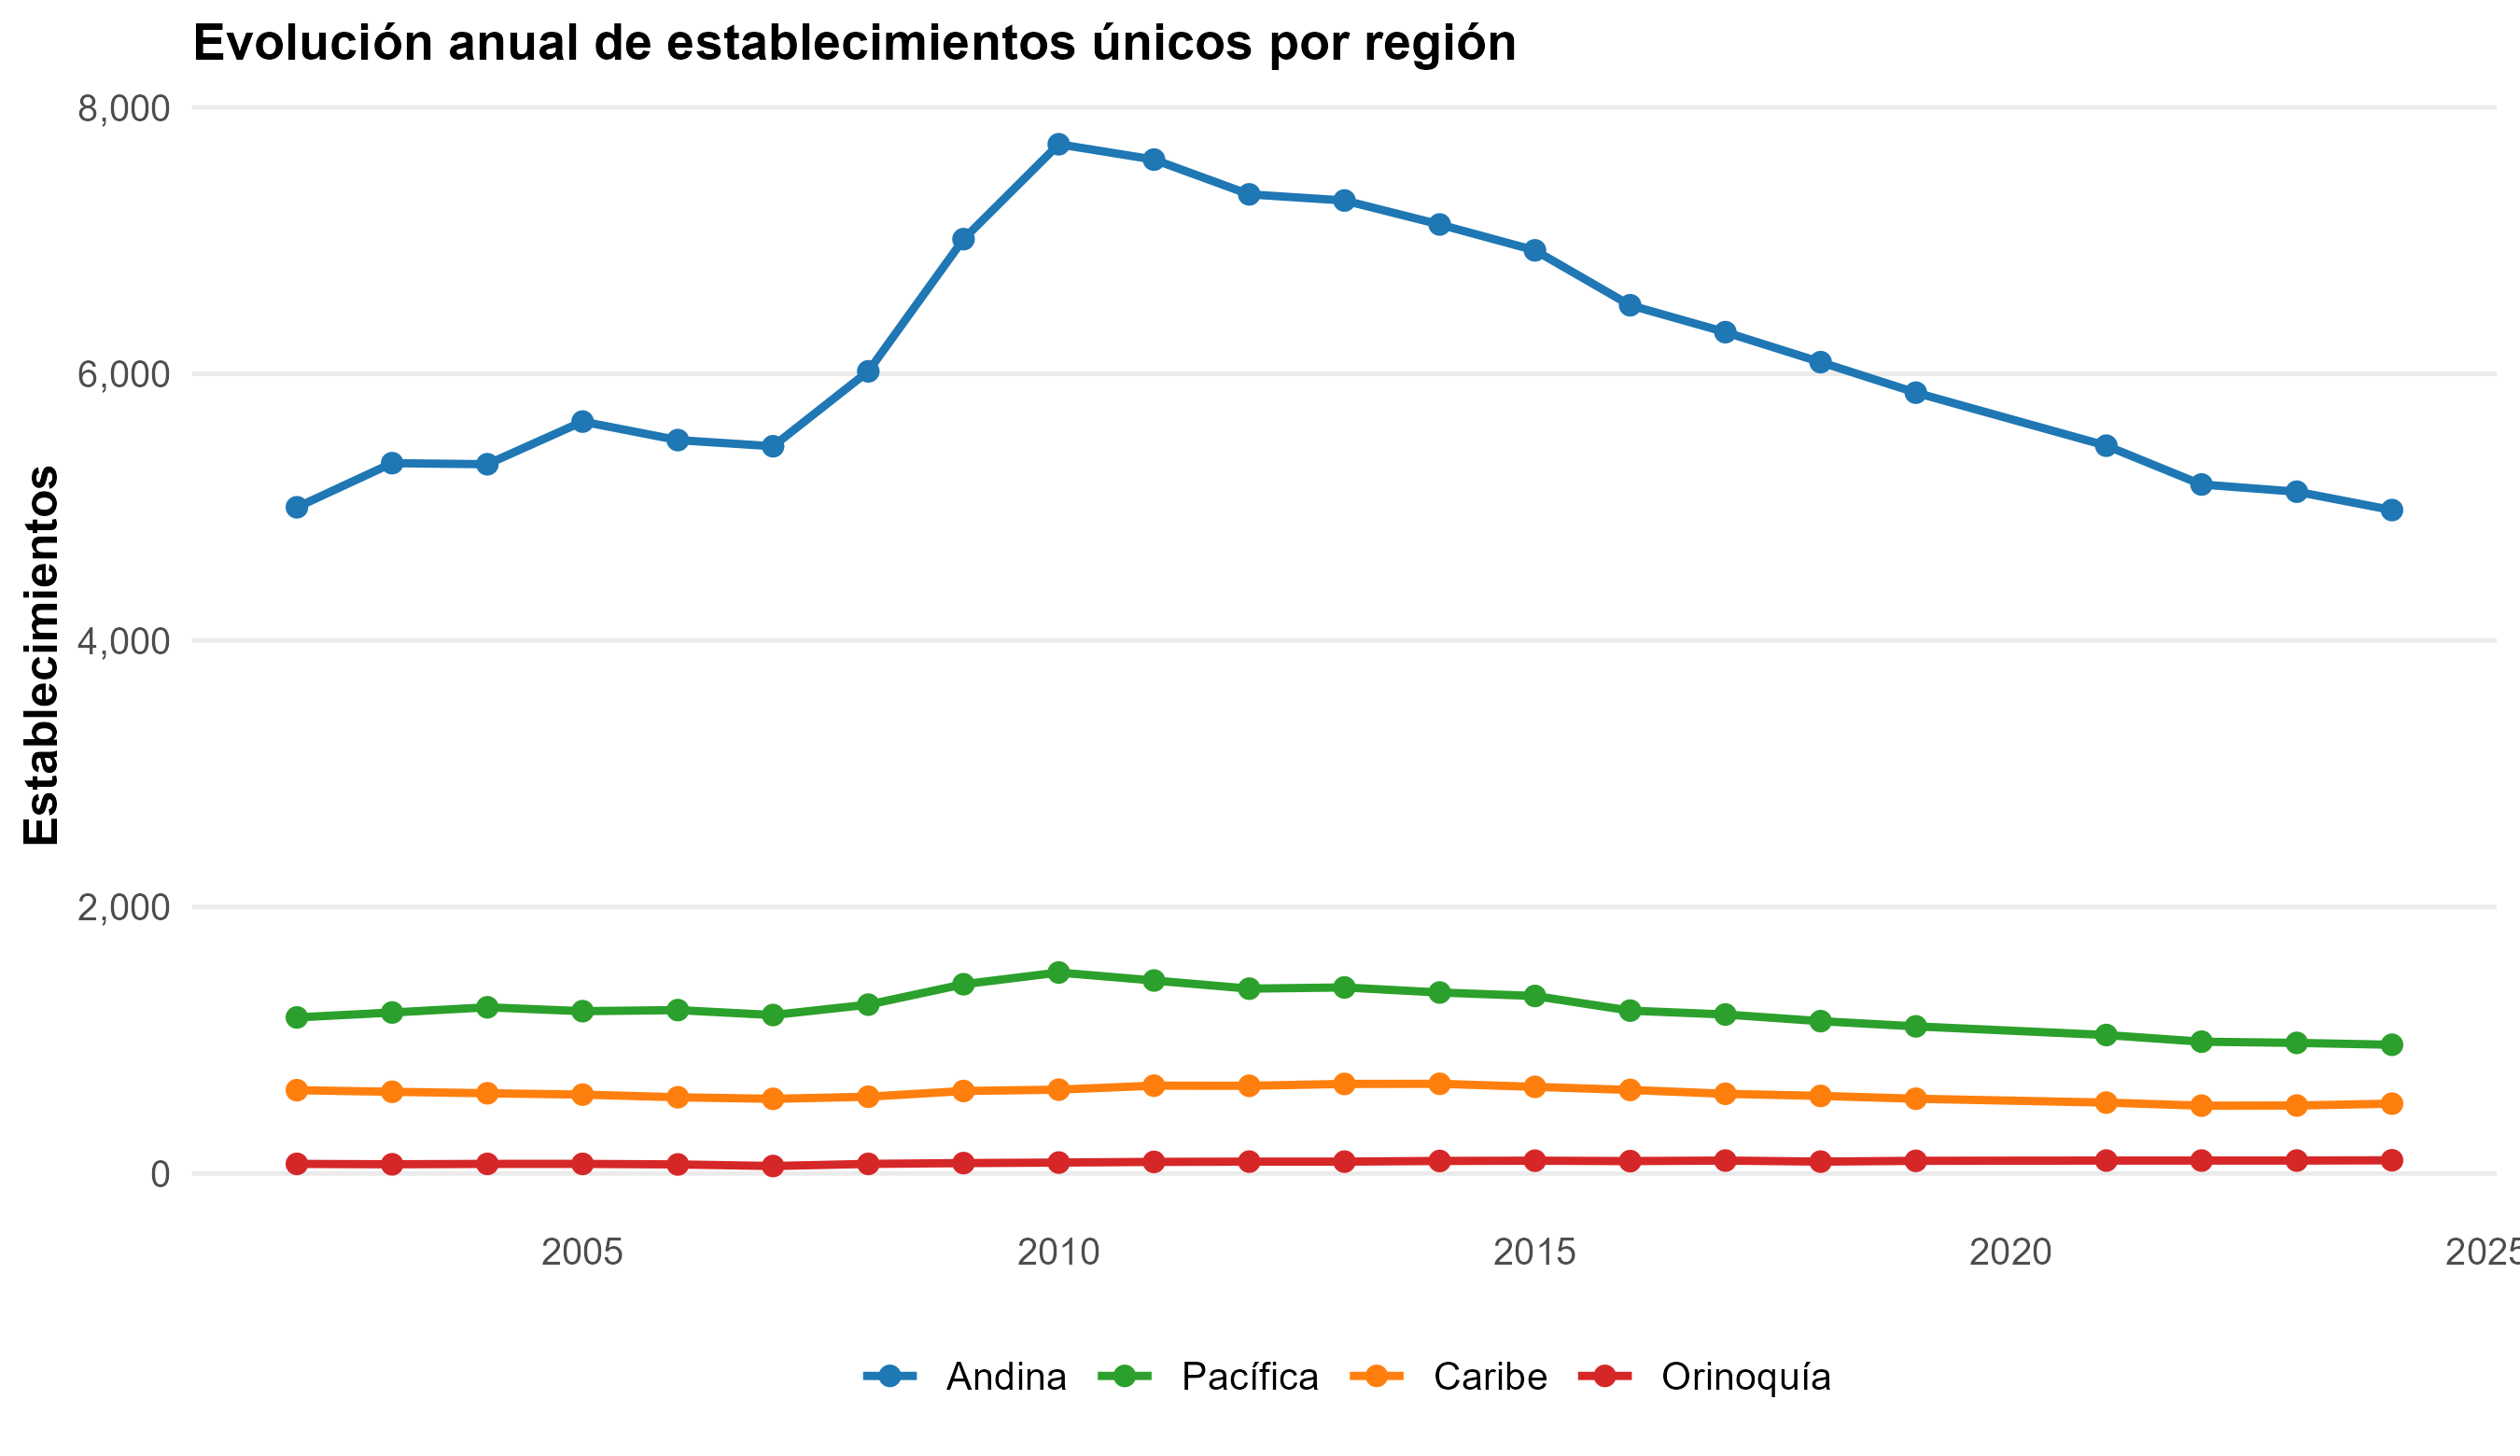
\includegraphics[width=0.9\linewidth]{fig7.png}
\end{frame}

\begin{frame}{Participacion por region}
  \centering
  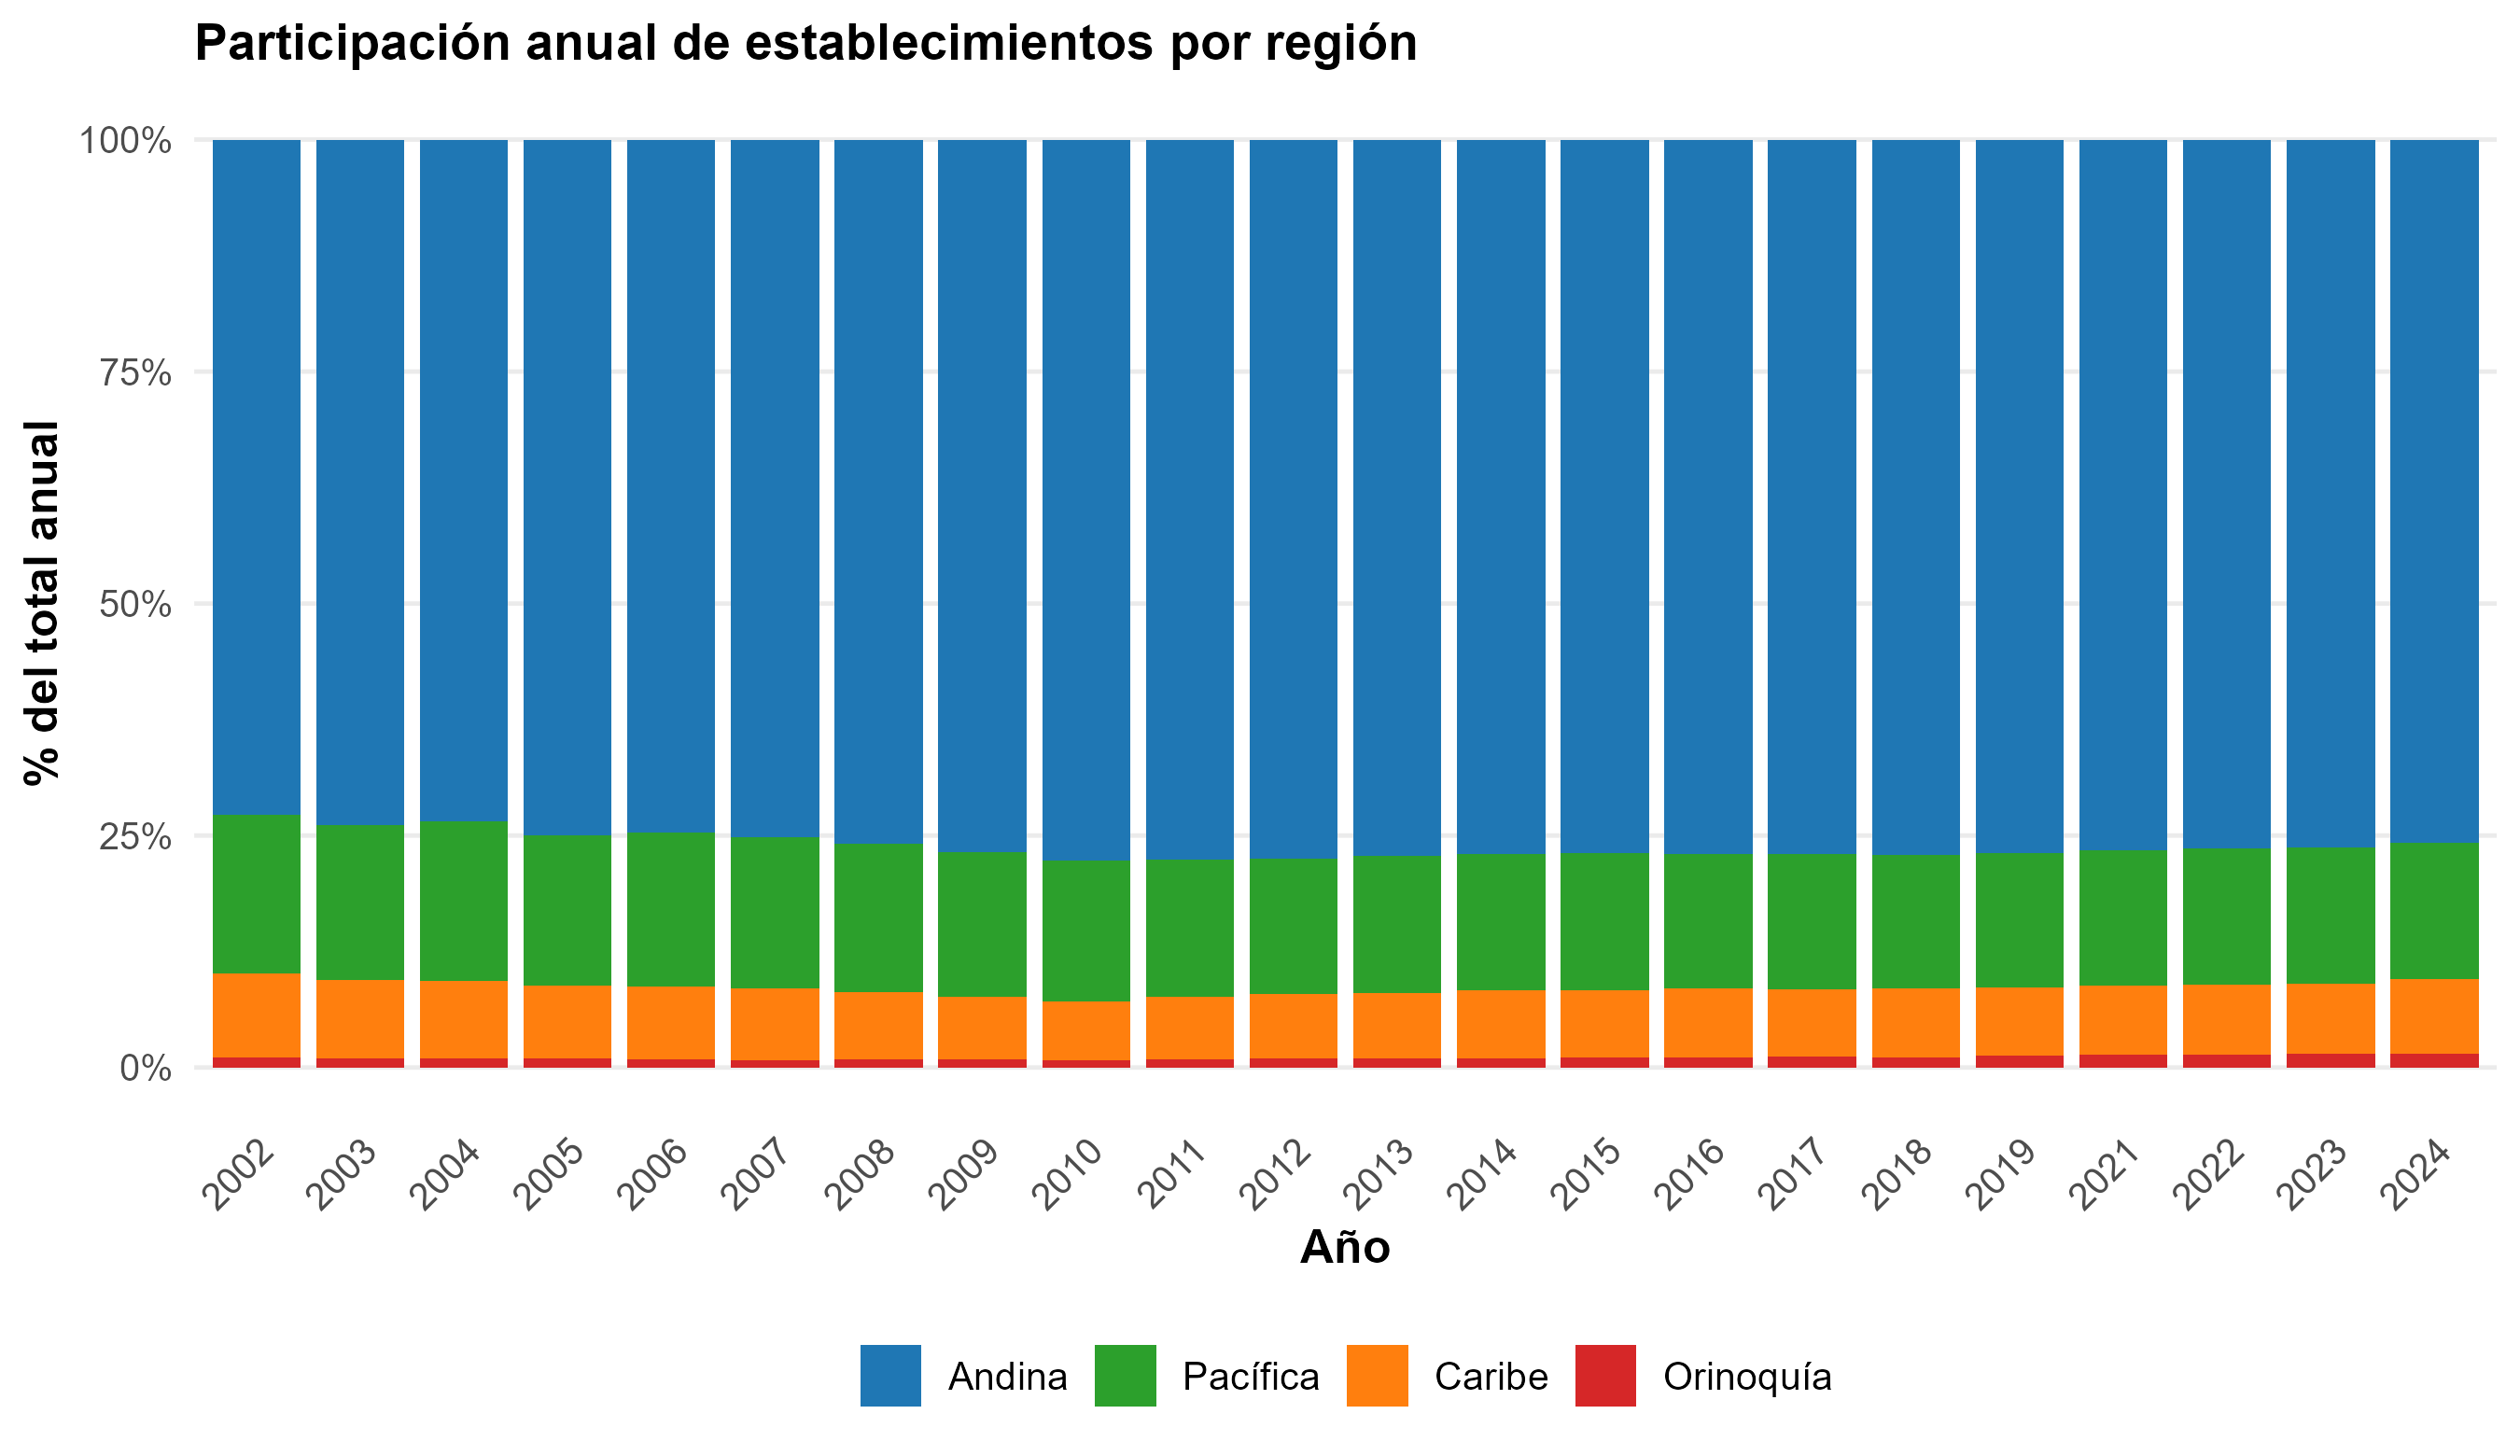
\includegraphics[width=0.9\linewidth]{fig8.png}
\end{frame}

\begin{frame}{Valor agregado por region}
  \centering
  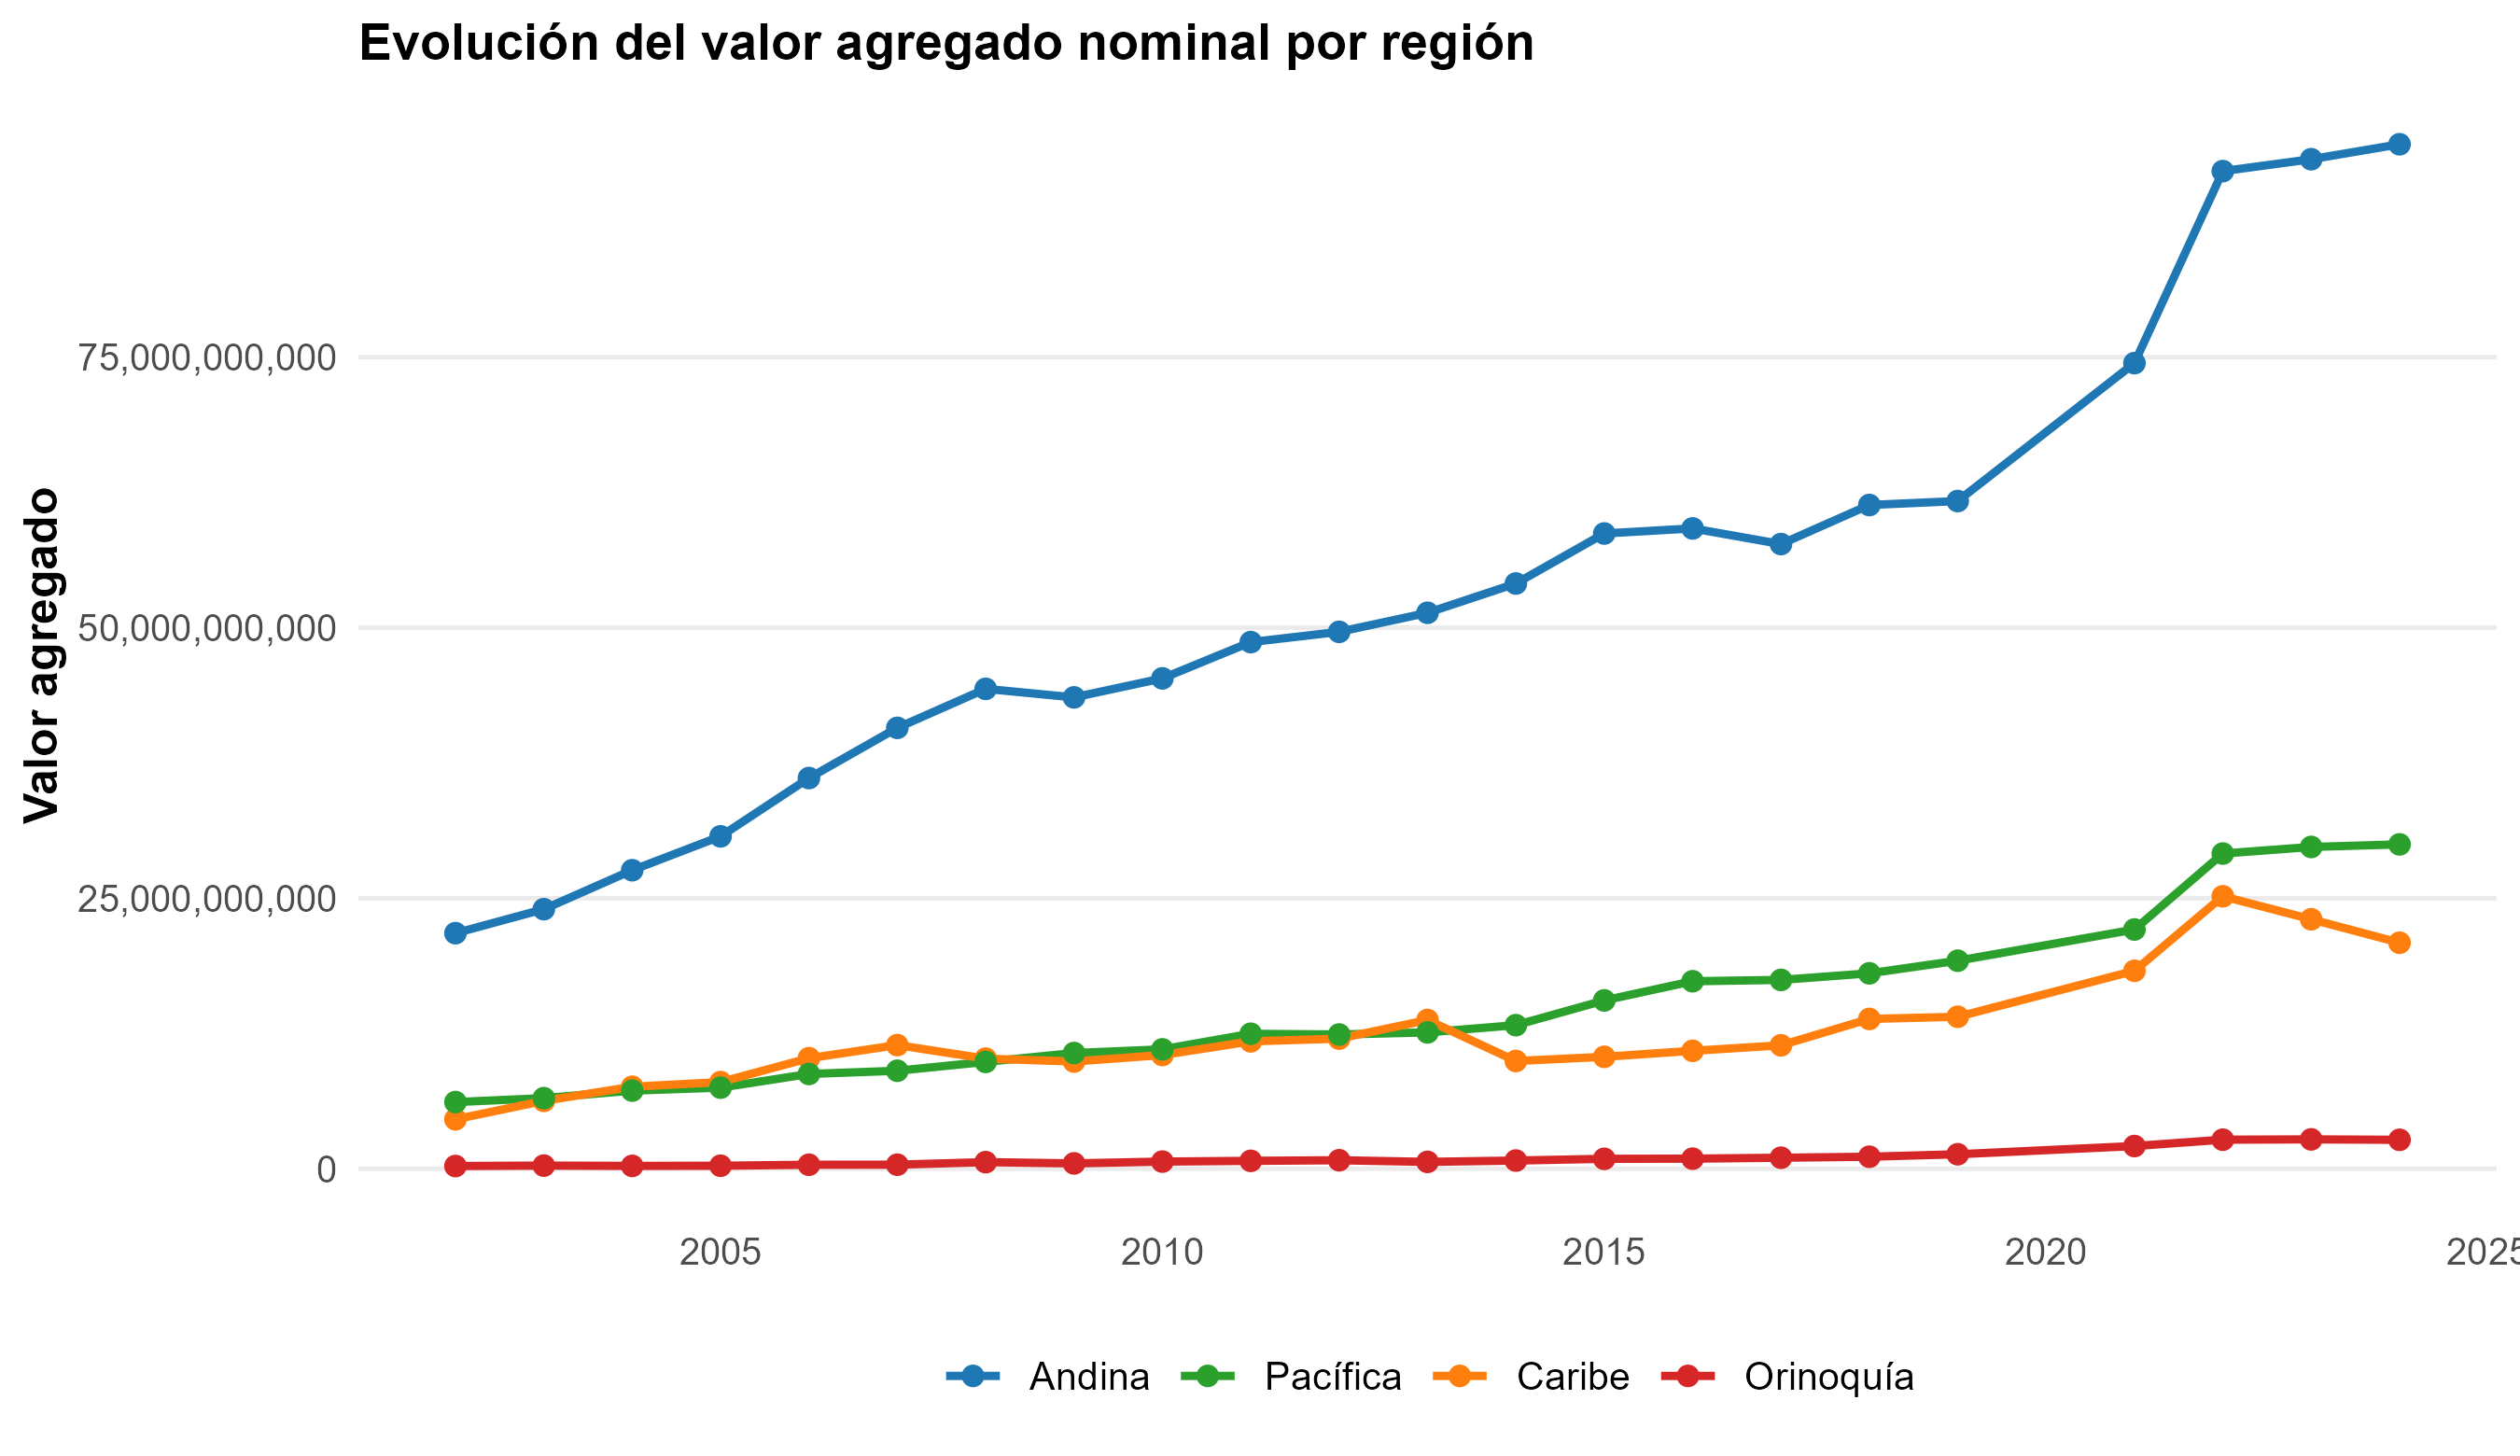
\includegraphics[width=0.9\linewidth]{fig9.png}
\end{frame}

\begin{frame}{Personal ocupado por region}
  \centering
  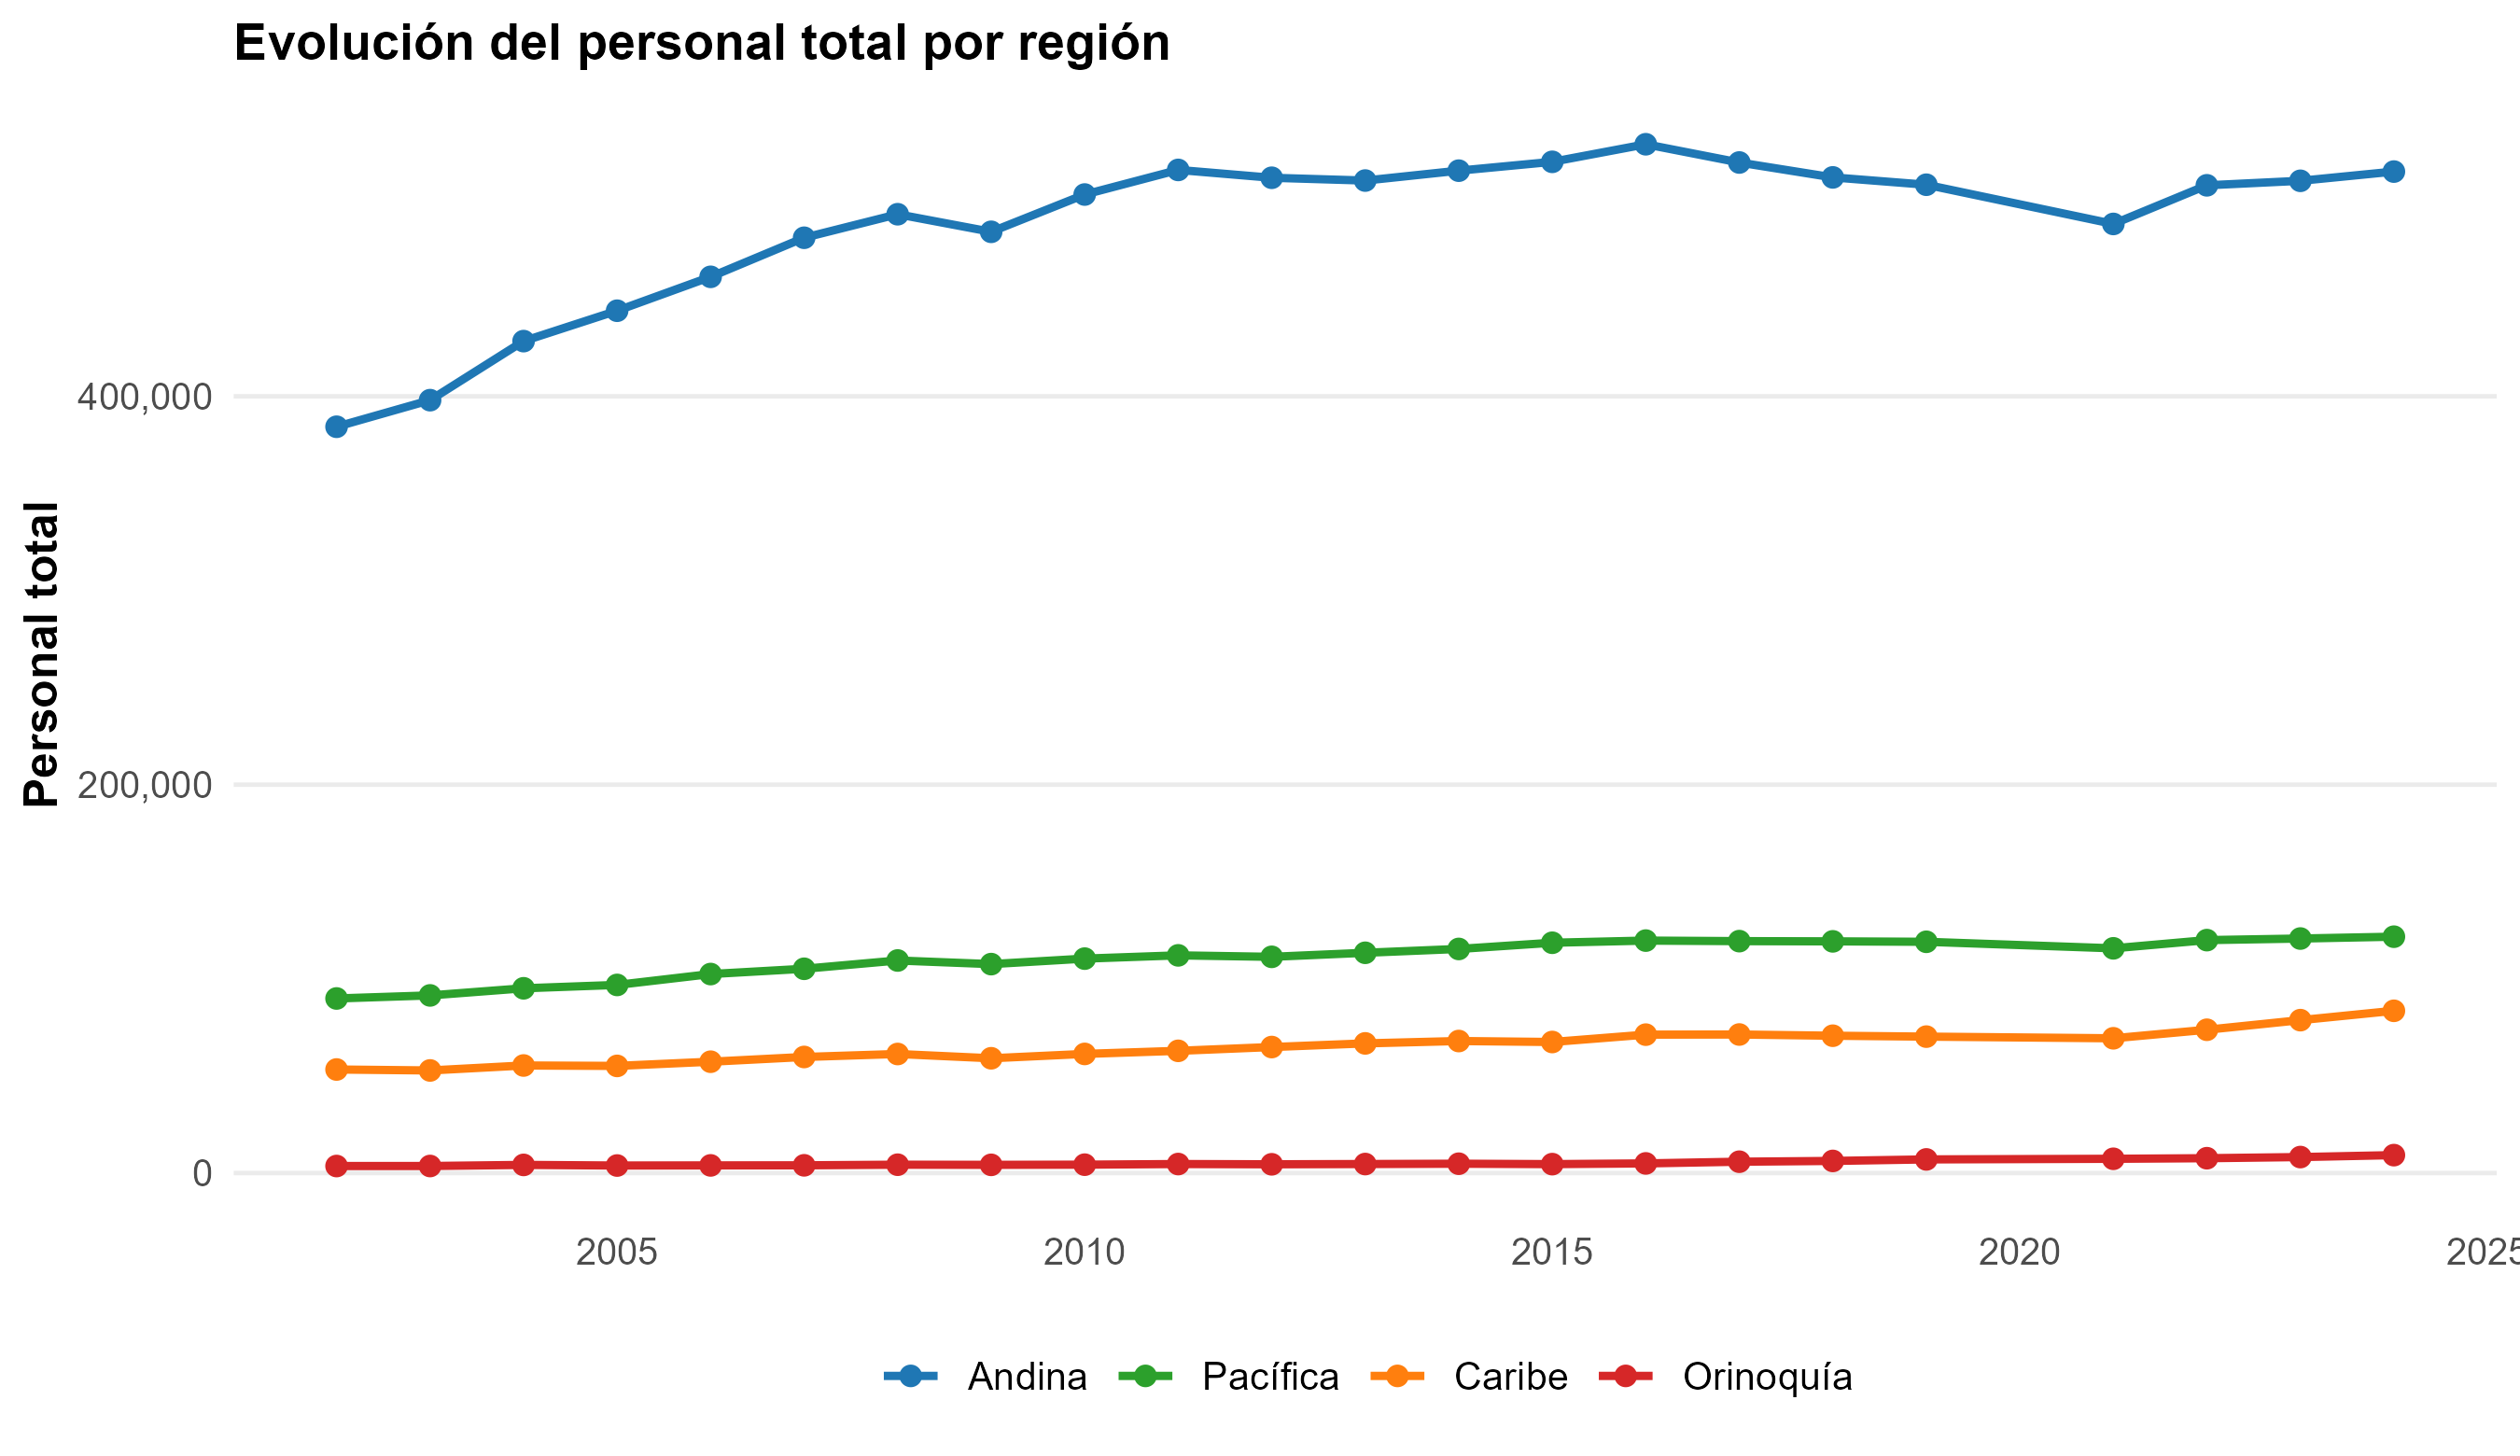
\includegraphics[width=0.9\linewidth]{fig10.png}
\end{frame}

\begin{frame}{Productividad por region}
  \centering
  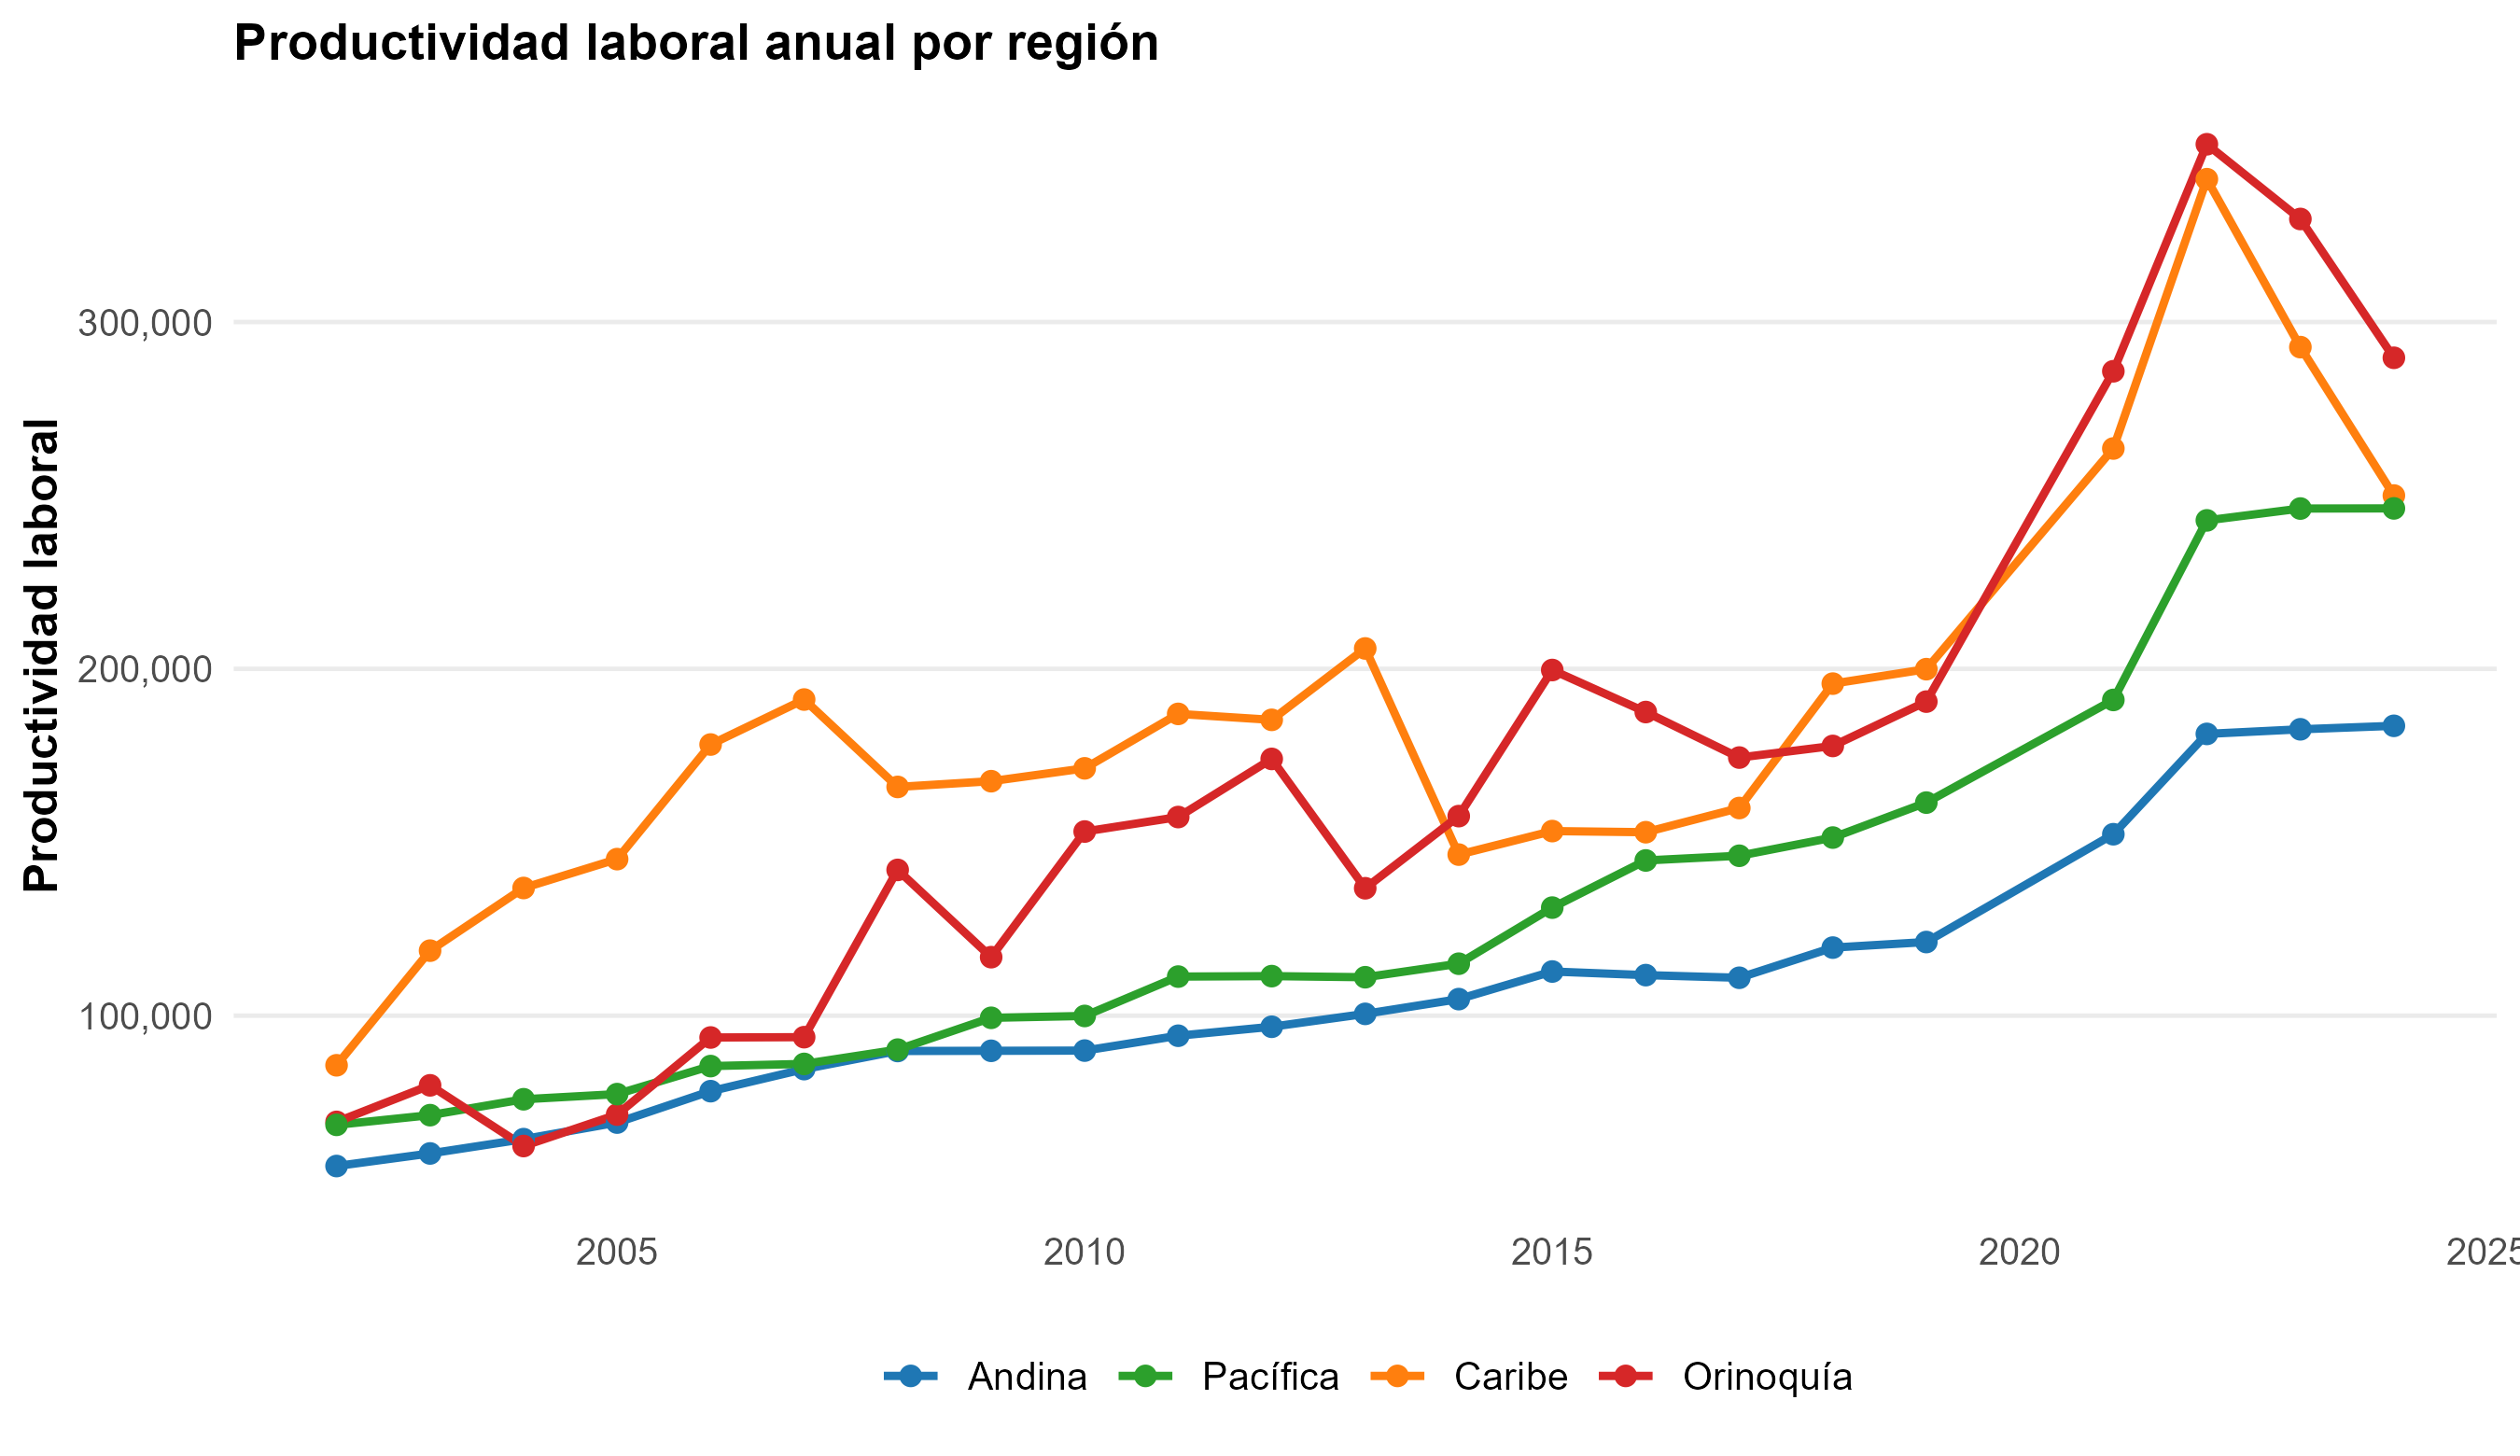
\includegraphics[width=0.9\linewidth]{fig11.png}
\end{frame}

\begin{frame}{Establecimientos por region y sector}
  \centering
  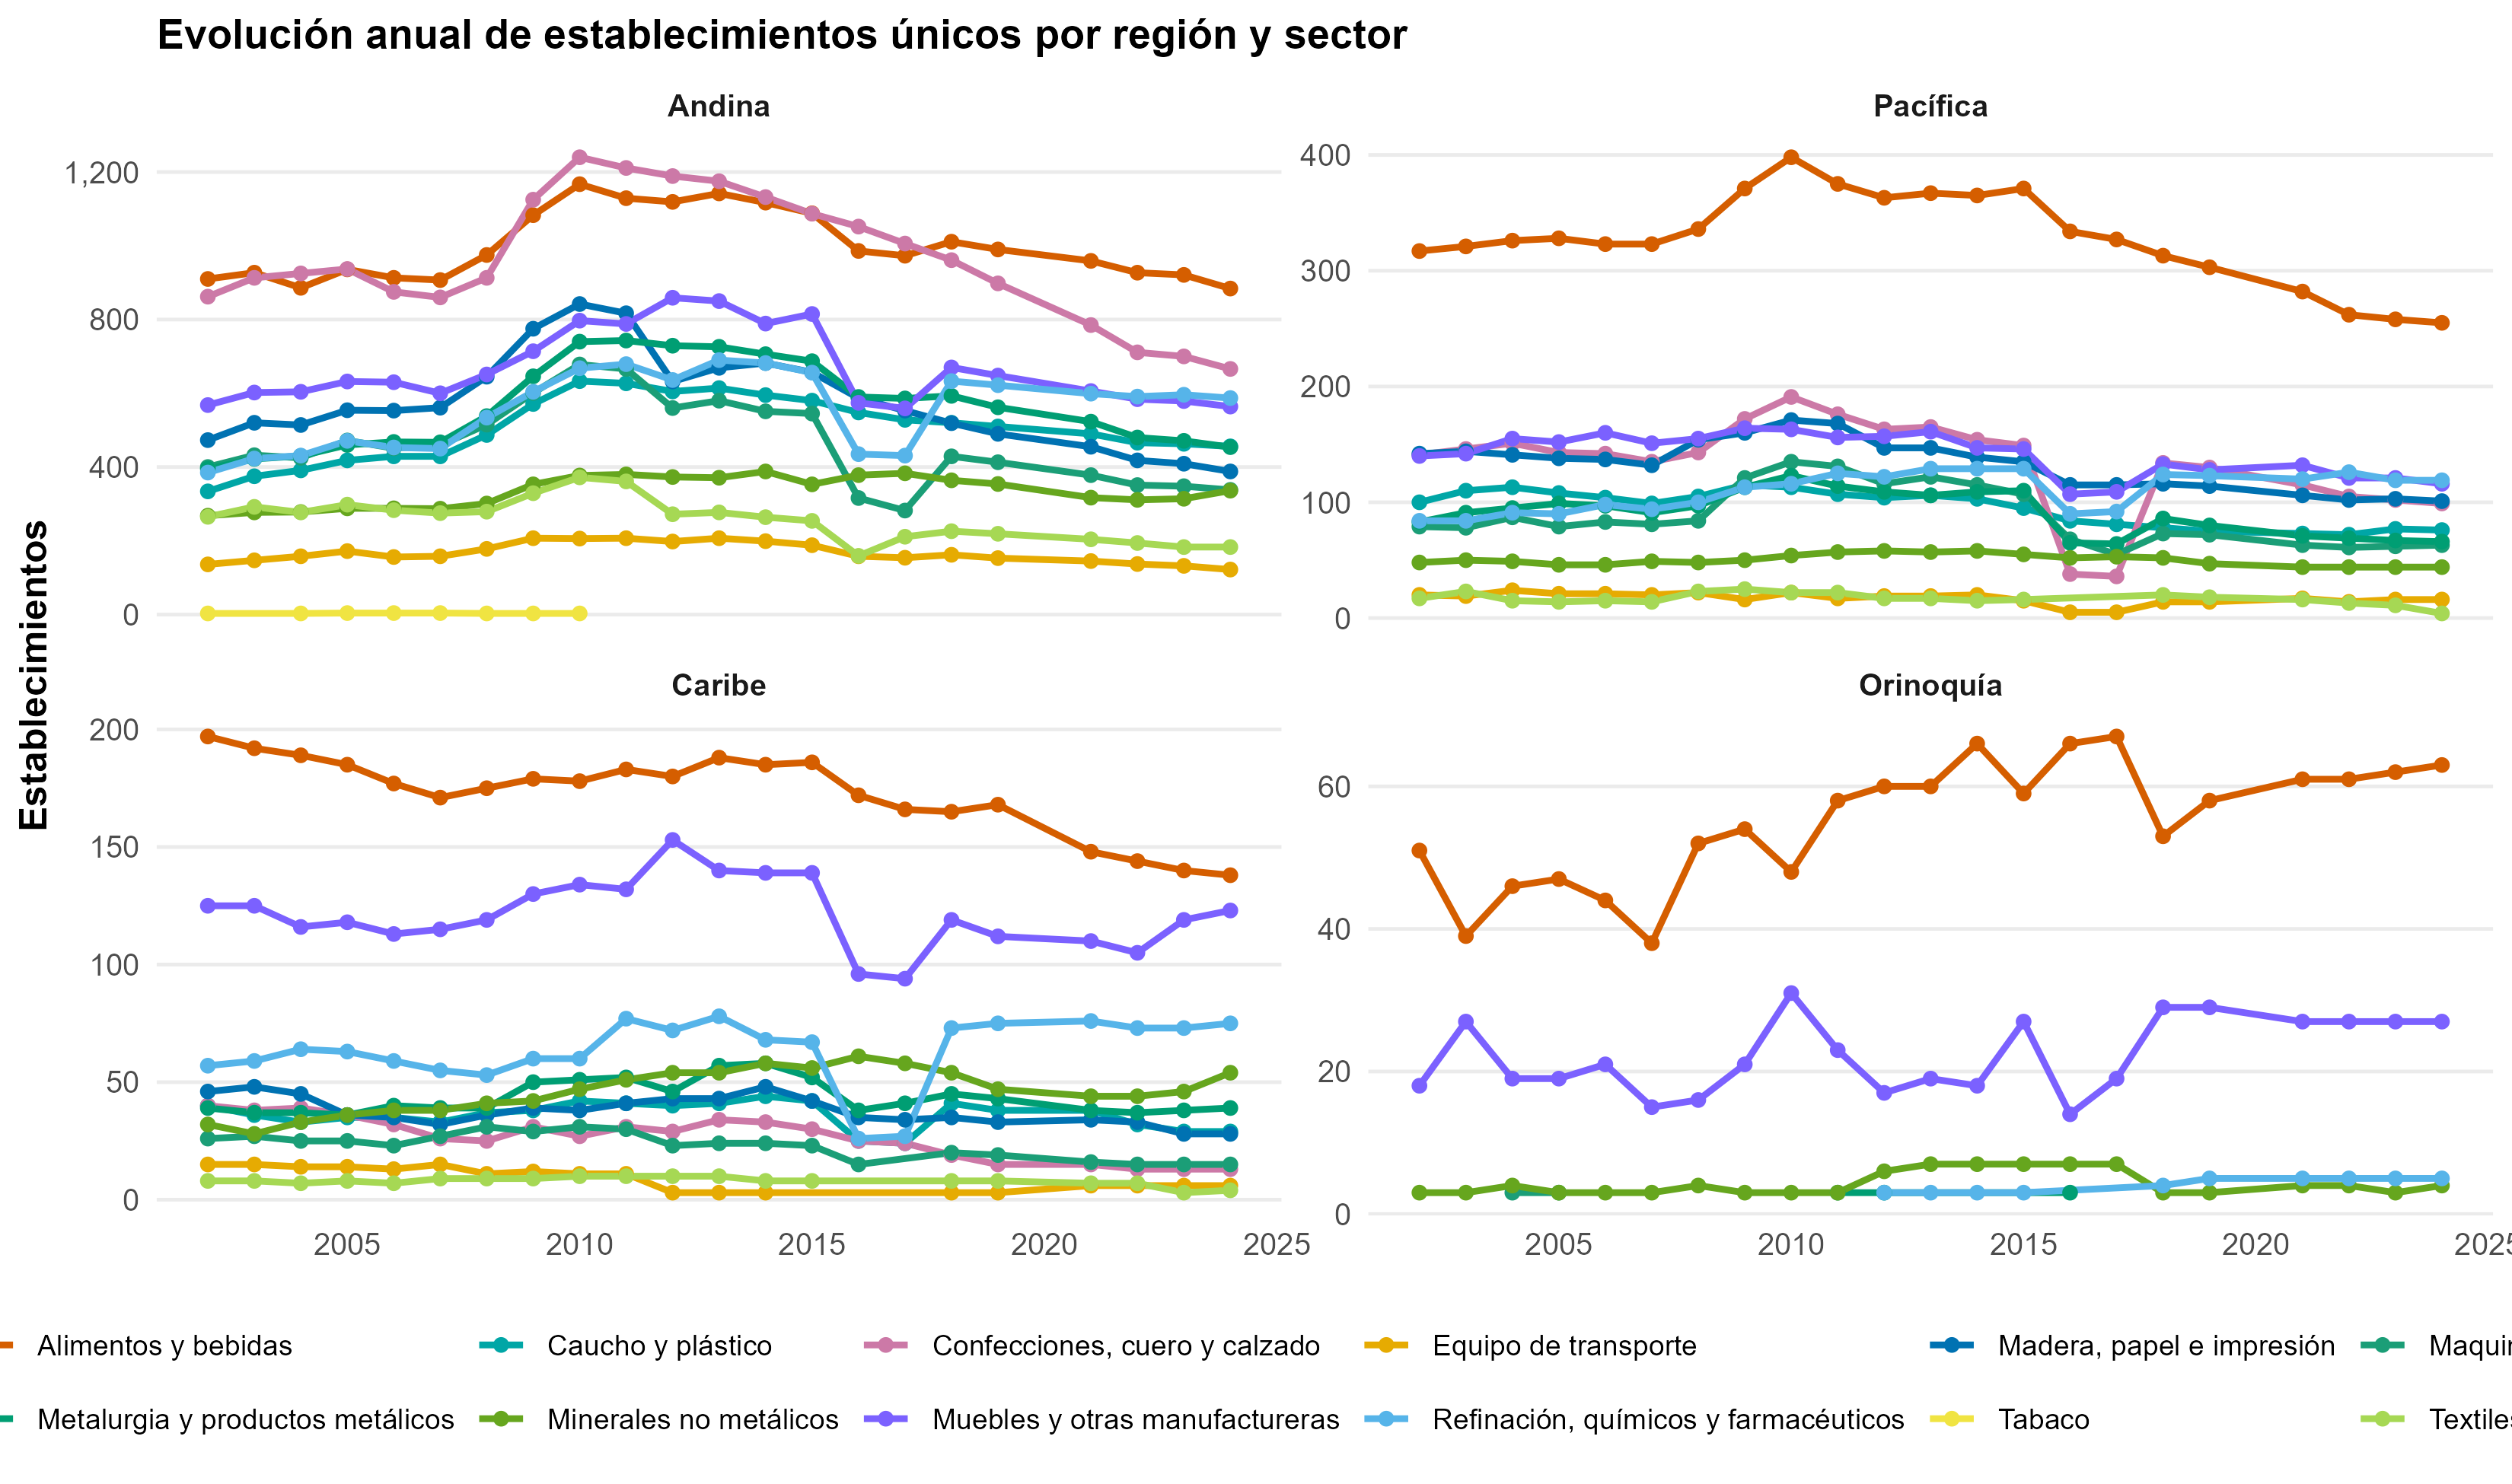
\includegraphics[width=0.9\linewidth]{fig12.png}
\end{frame}

\begin{frame}{Participacion por region y sector}
  \centering
  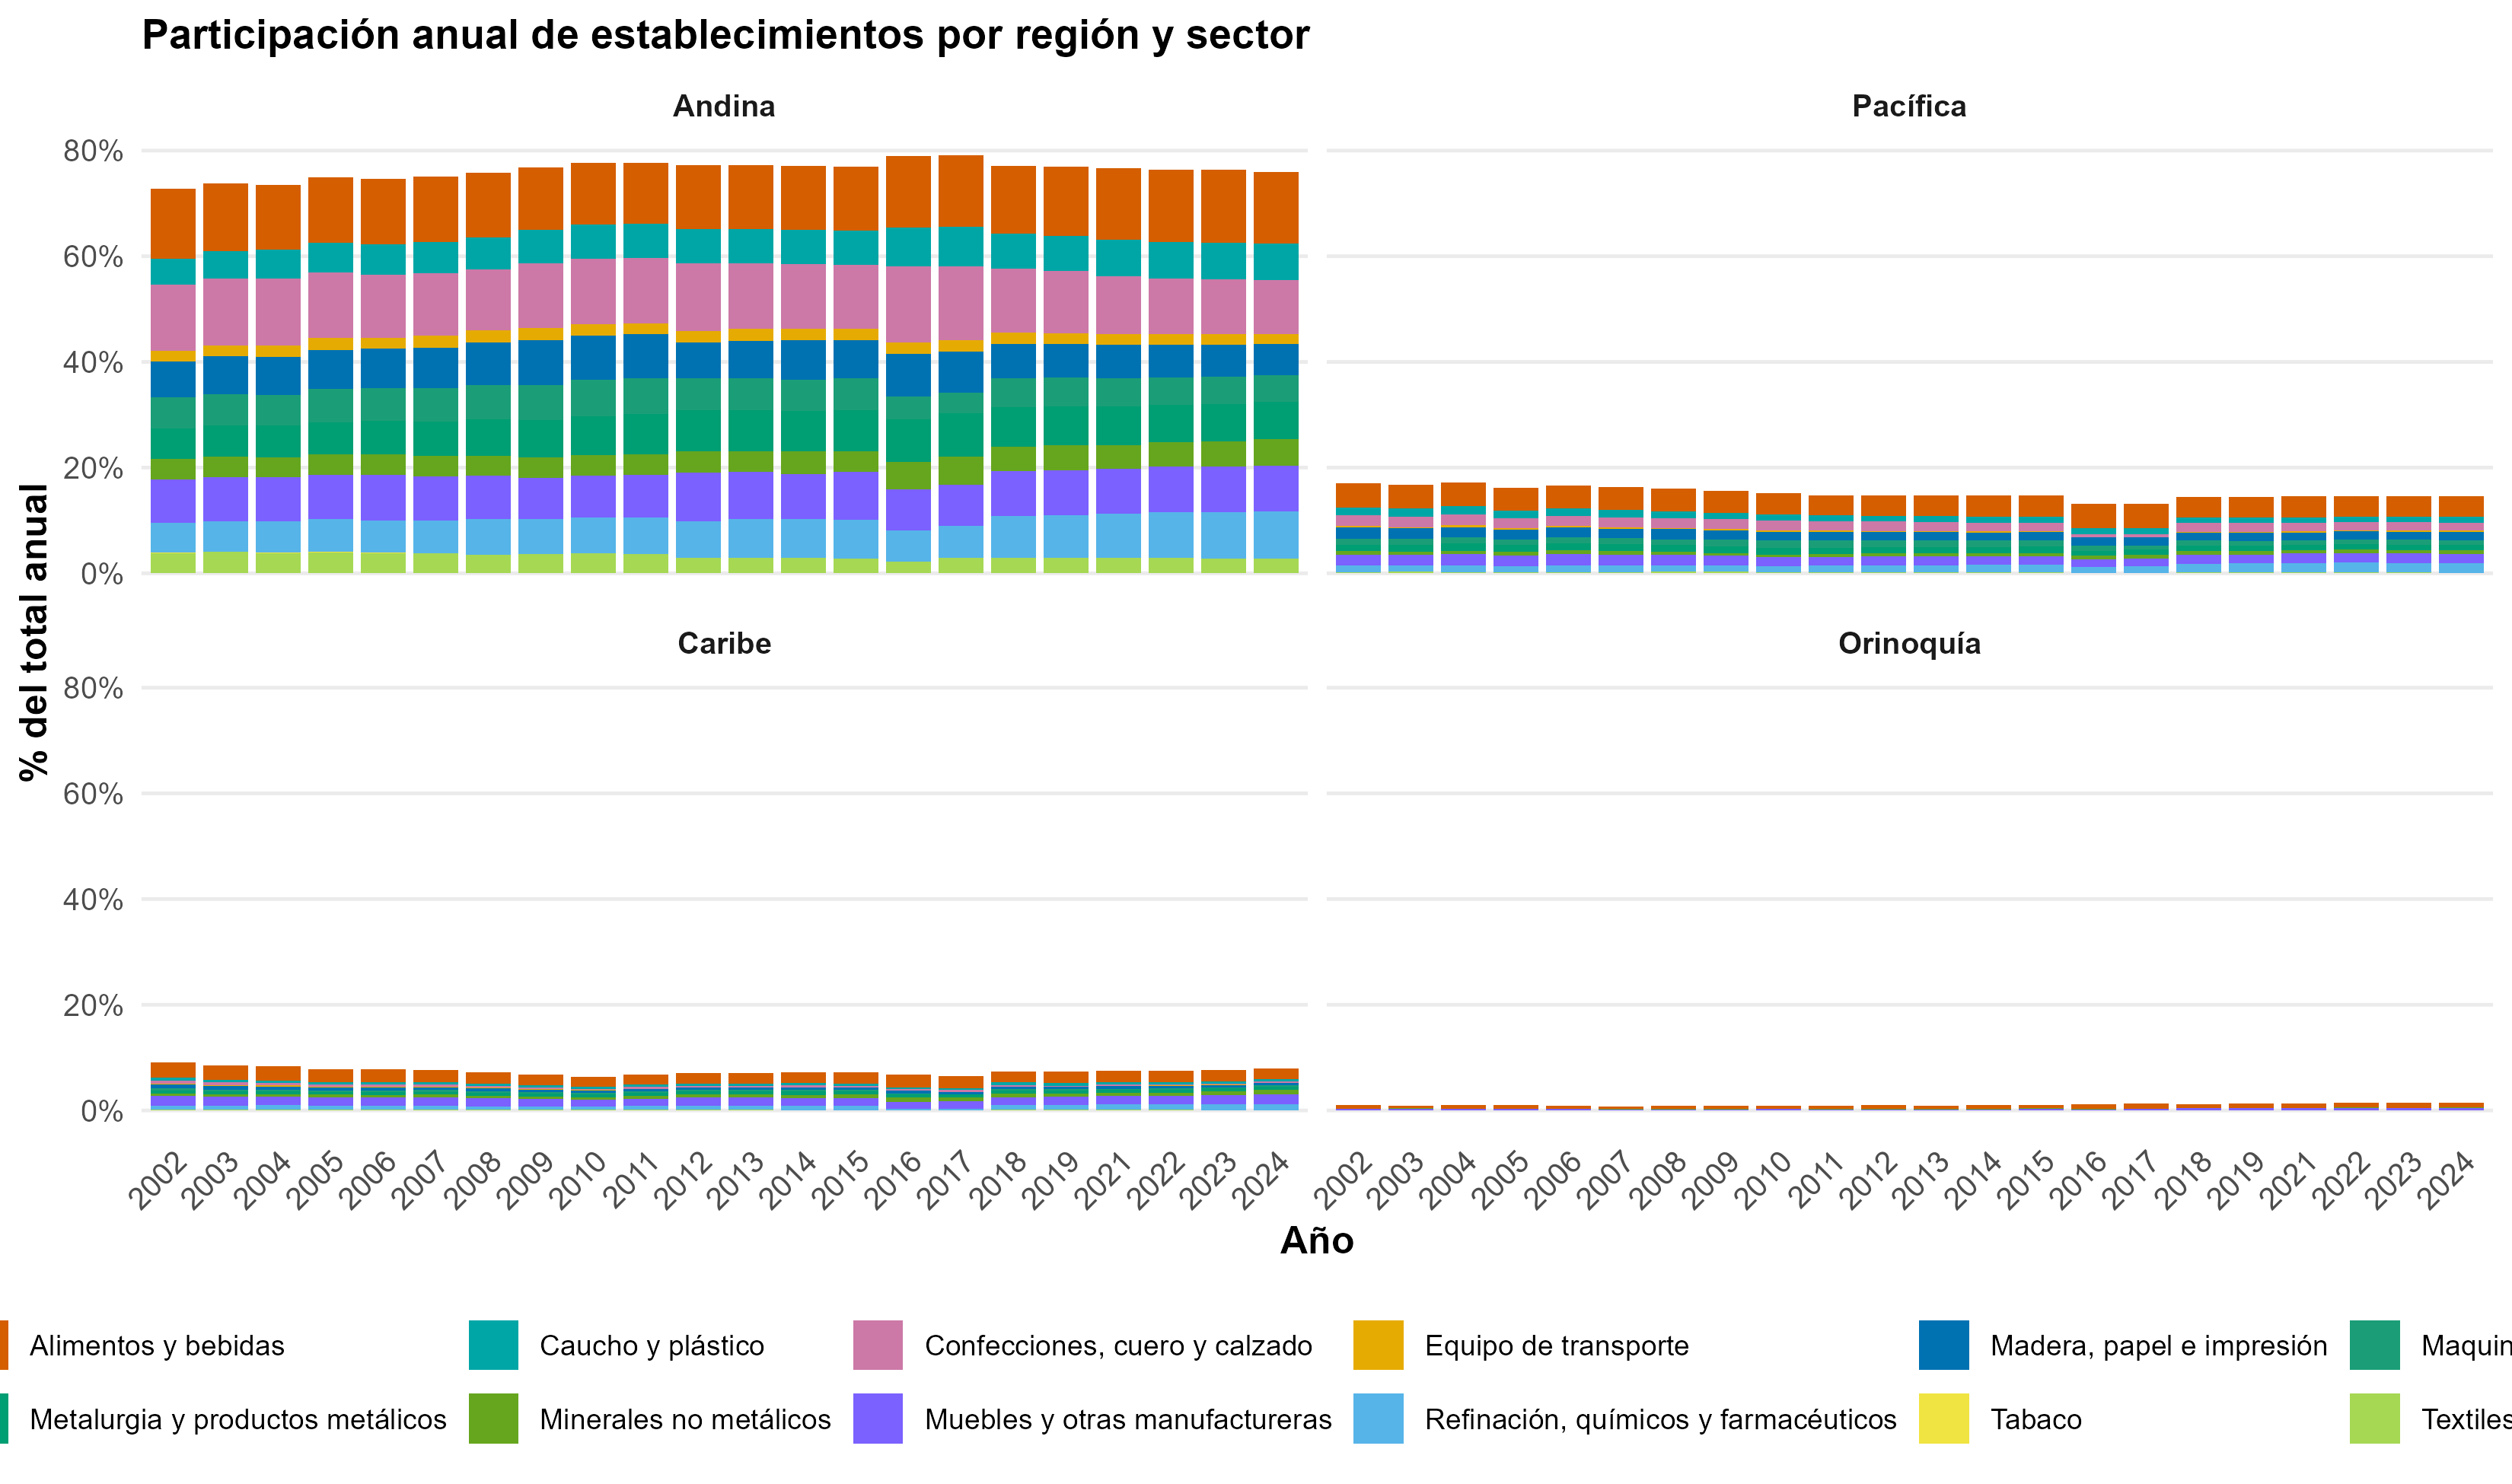
\includegraphics[width=0.9\linewidth]{fig12b_participacion_region_sector.png}
\end{frame}

\begin{frame}{Valor agregado por region y sector}
  \centering
  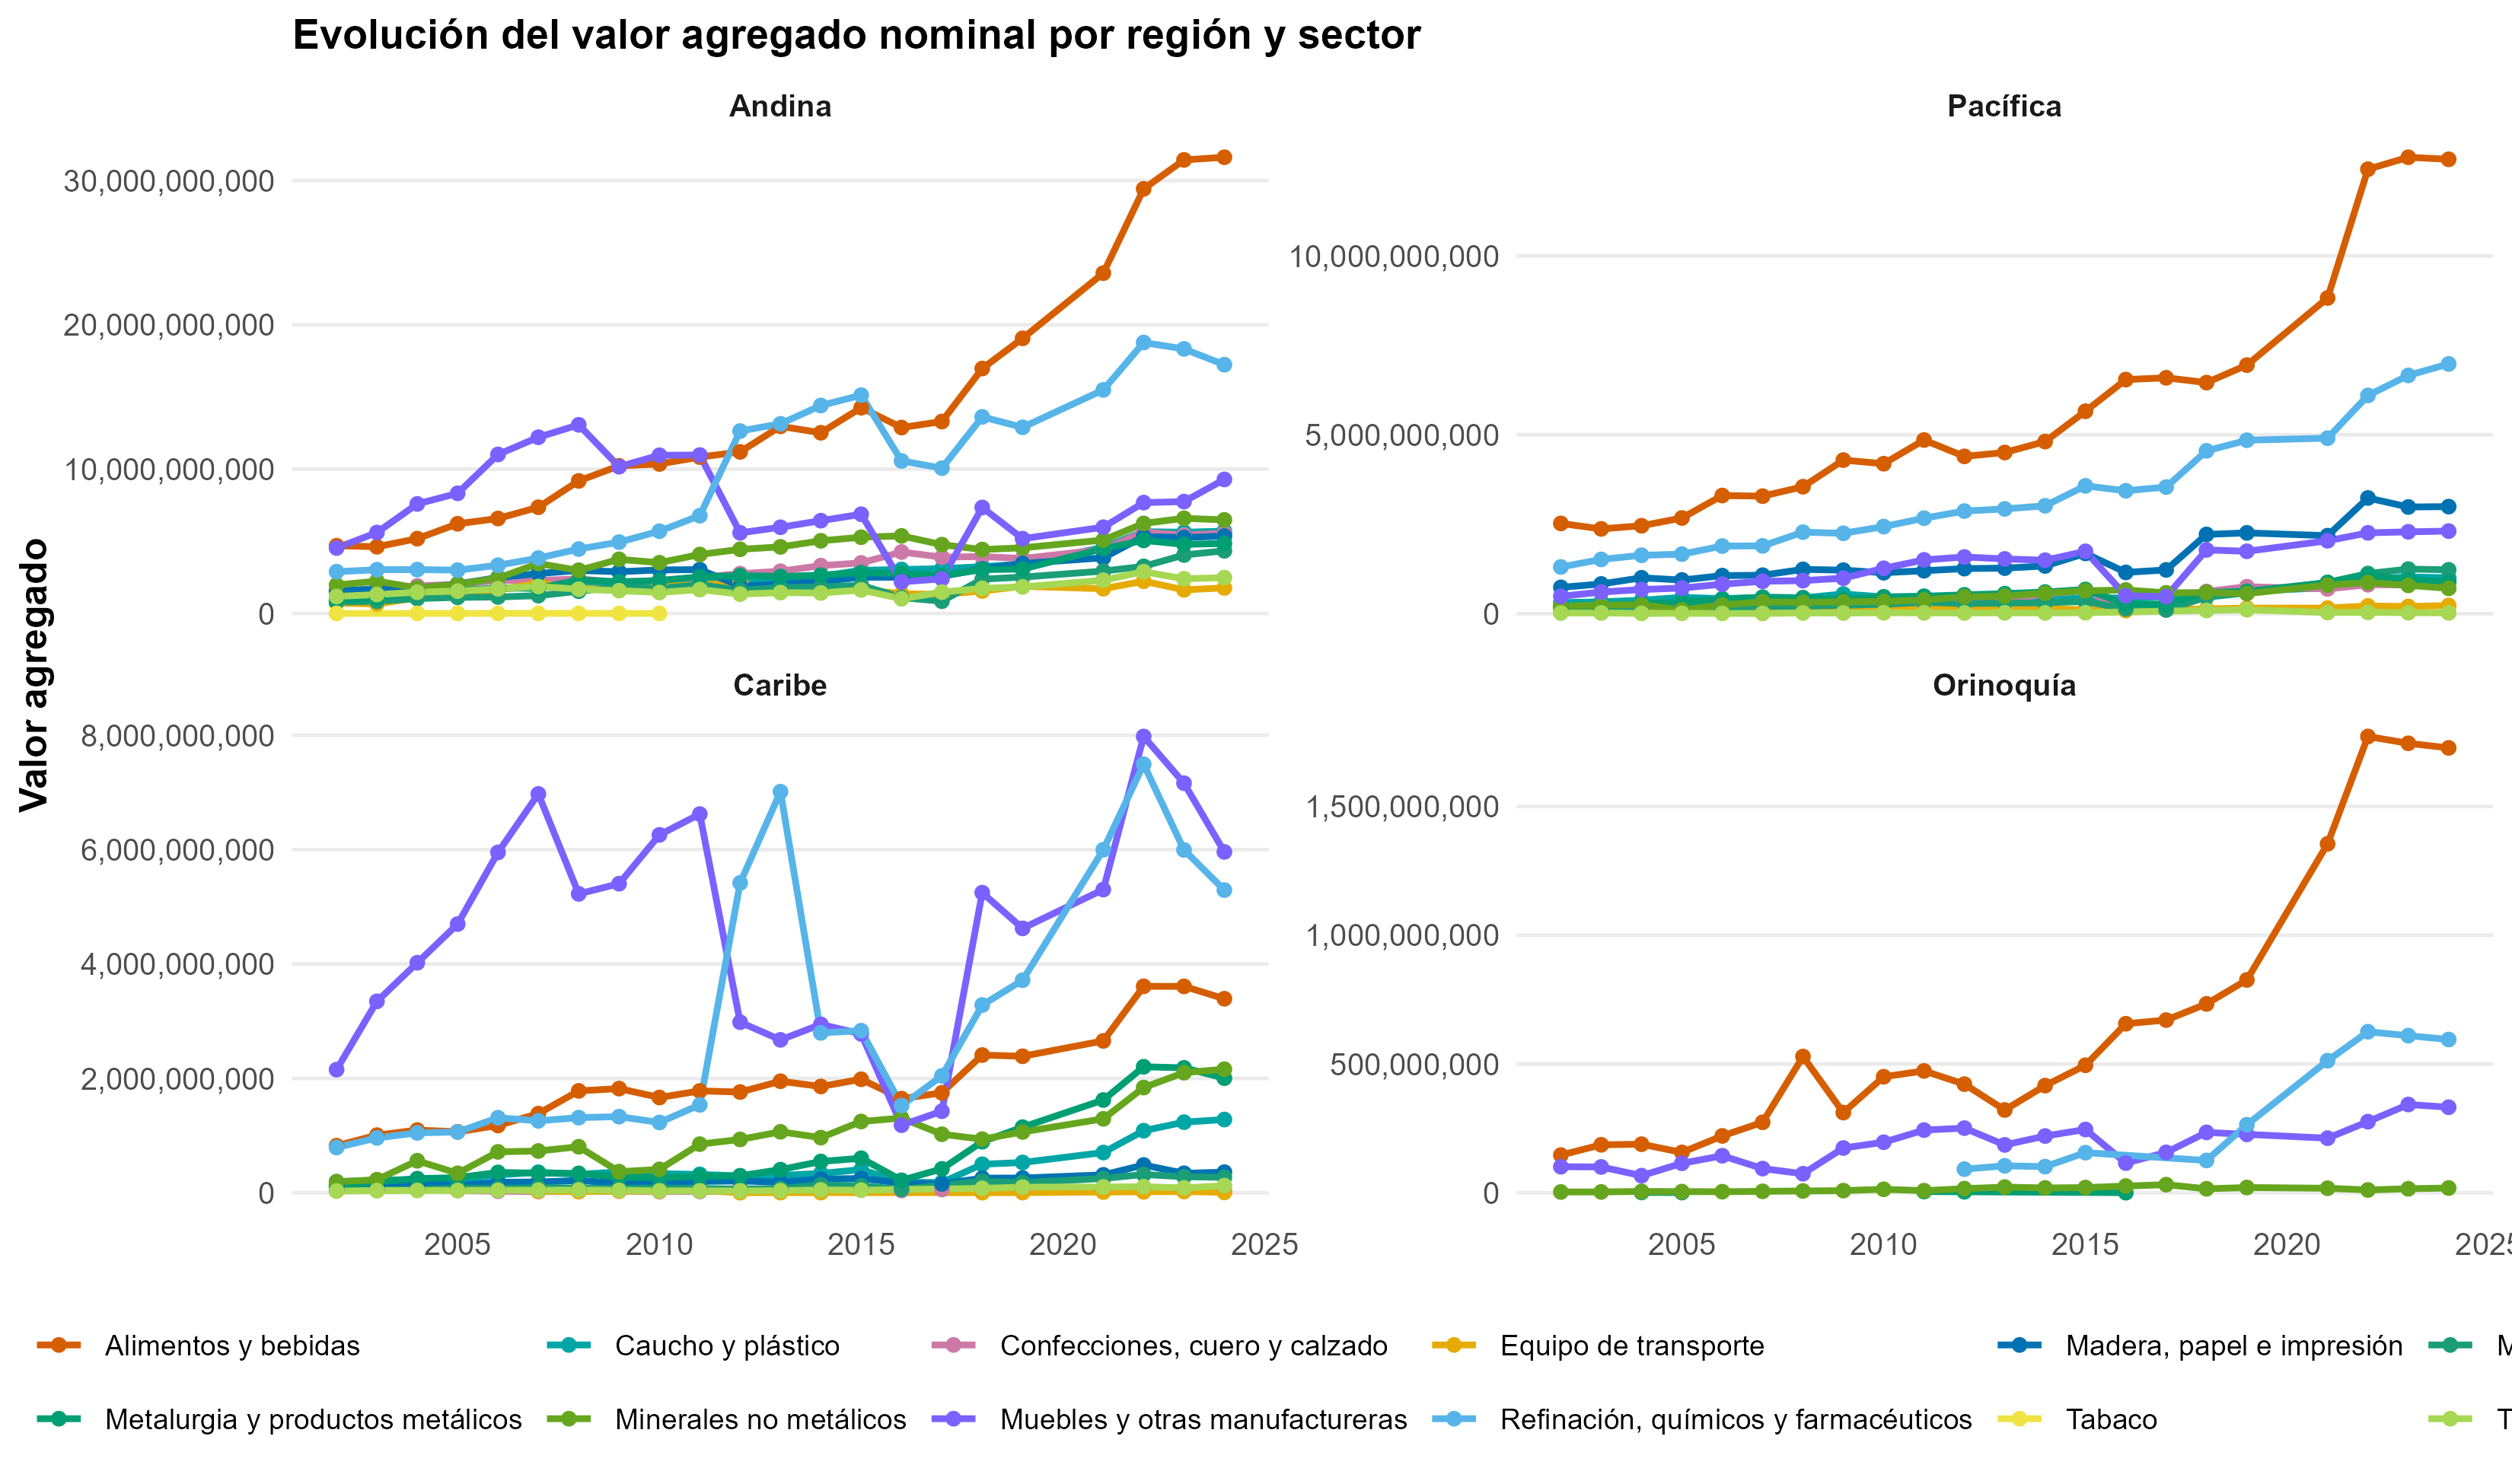
\includegraphics[width=0.9\linewidth]{fig13.png}
\end{frame}

\begin{frame}{Personal ocupado por region y sector}
  \centering
  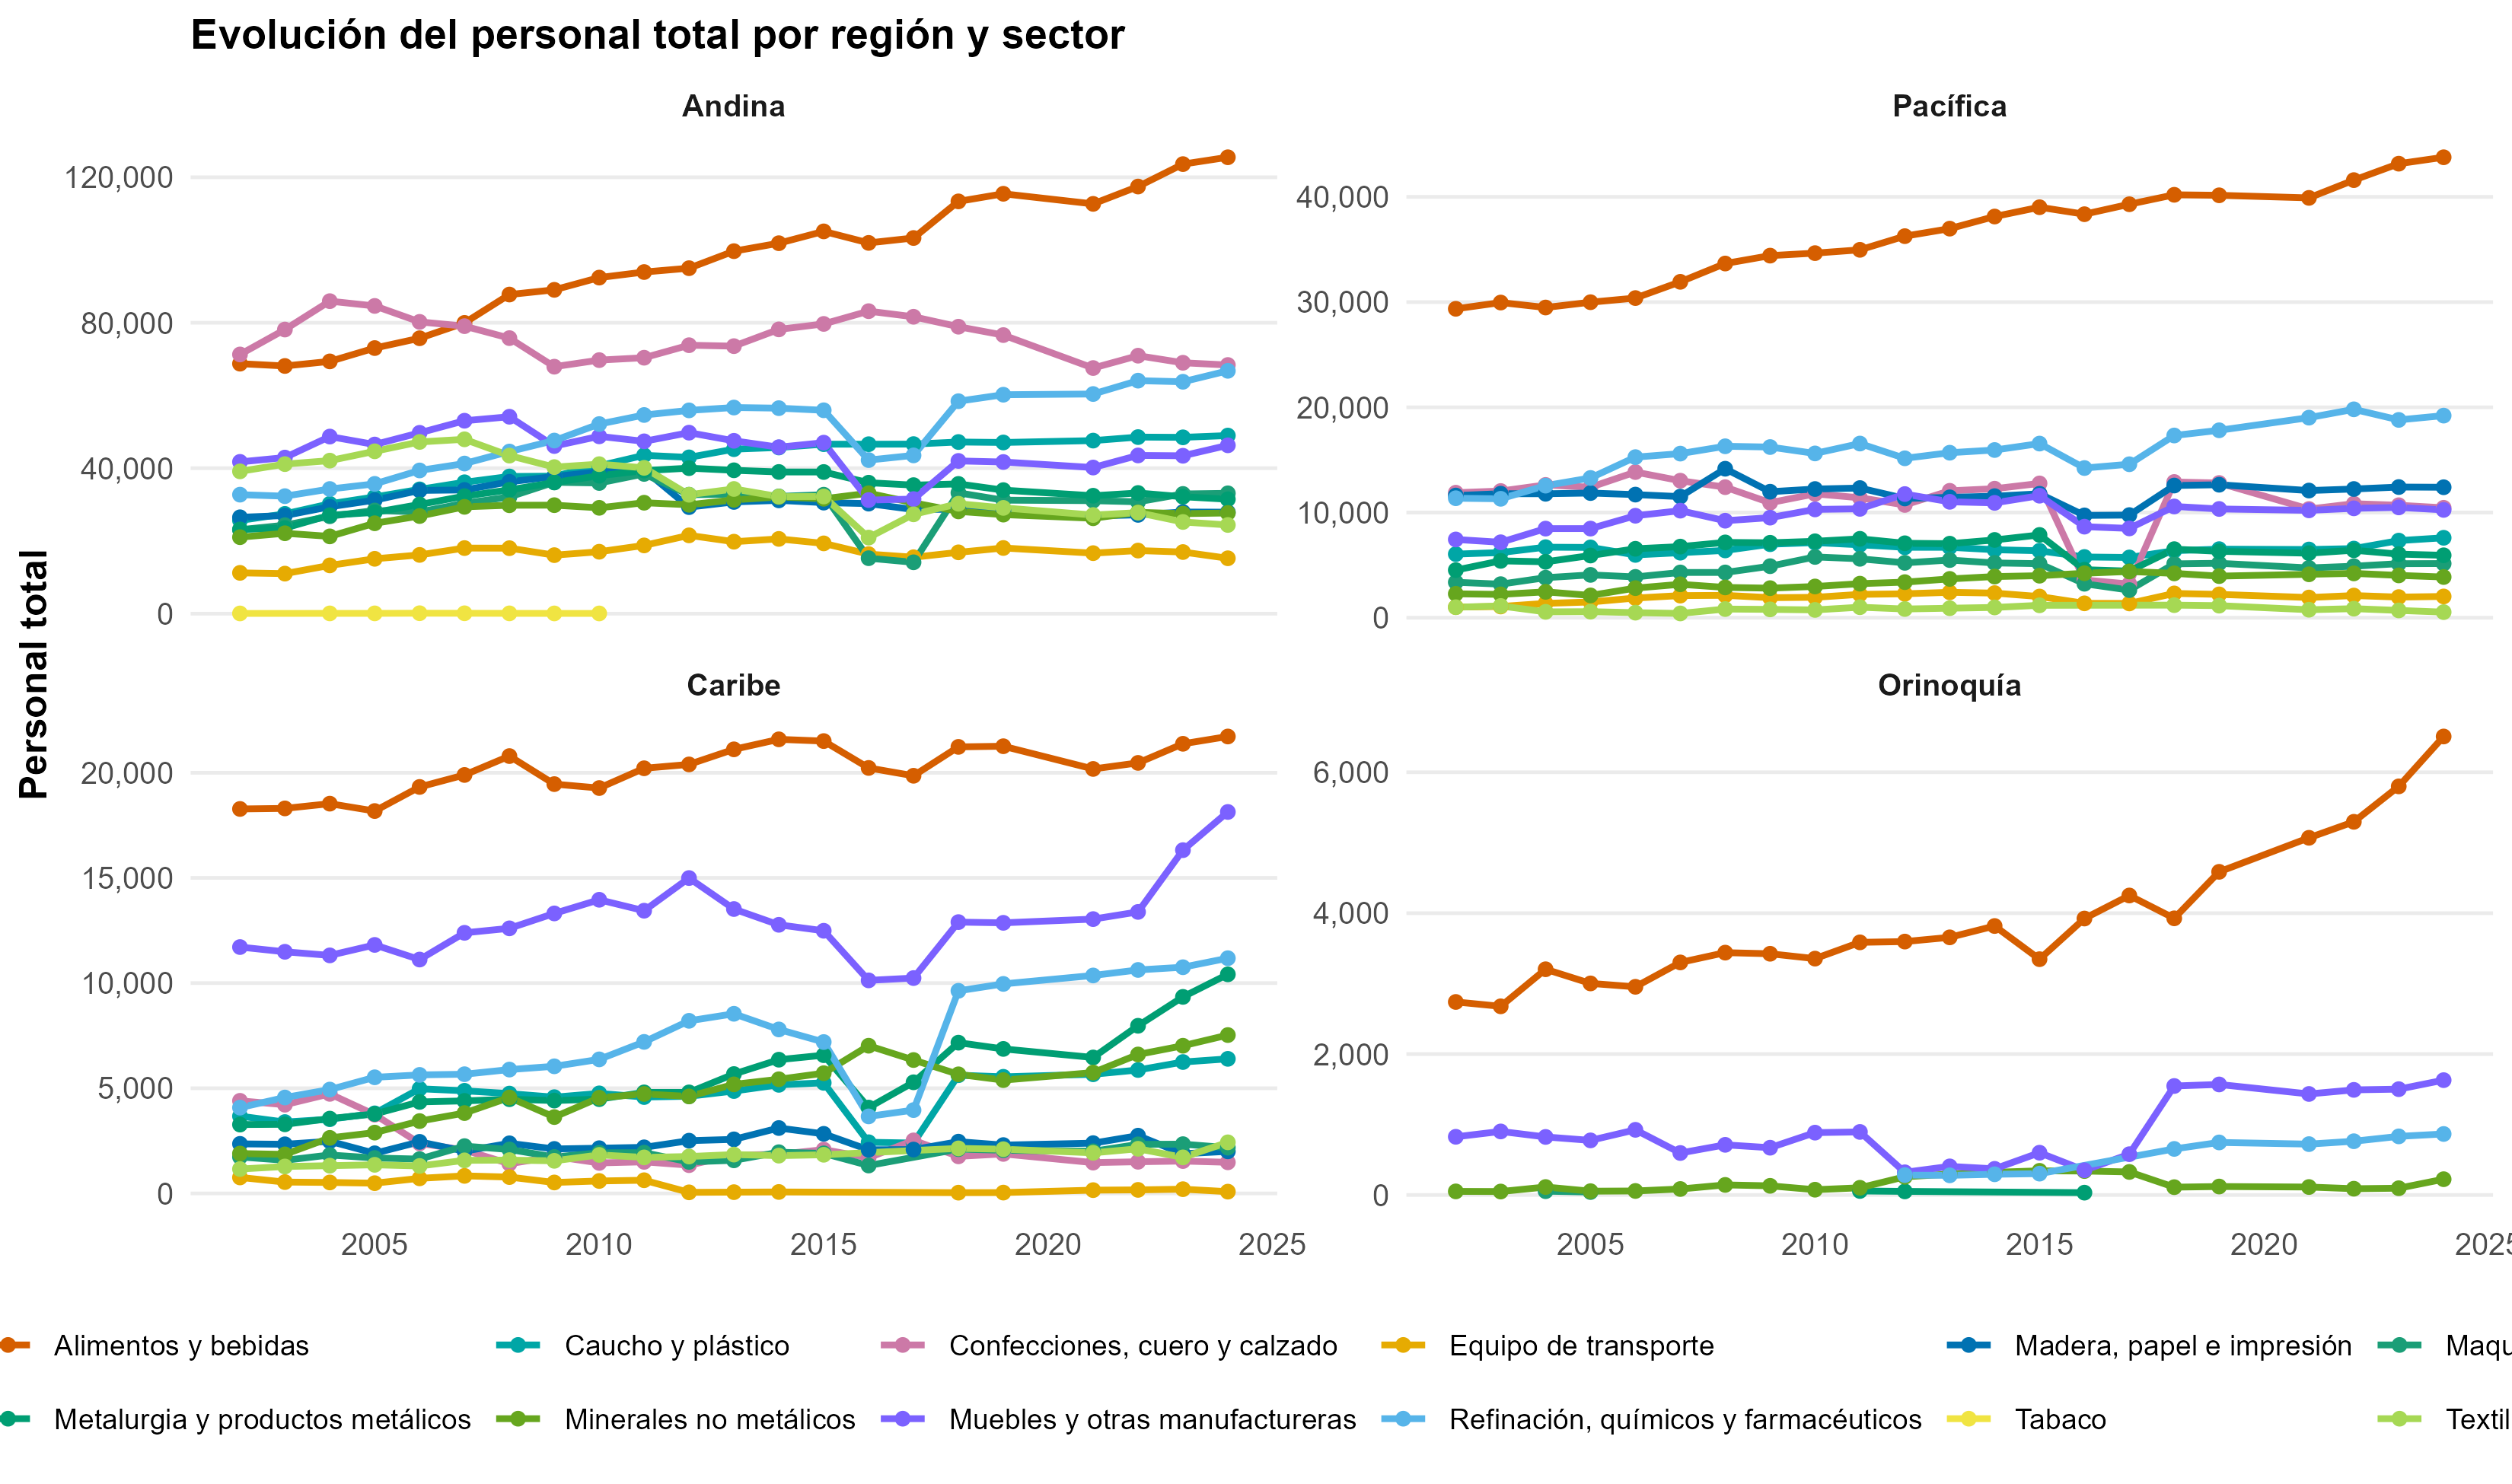
\includegraphics[width=0.9\linewidth]{fig14.png}
\end{frame}

\begin{frame}{Productividad por region y sector}
  \centering
  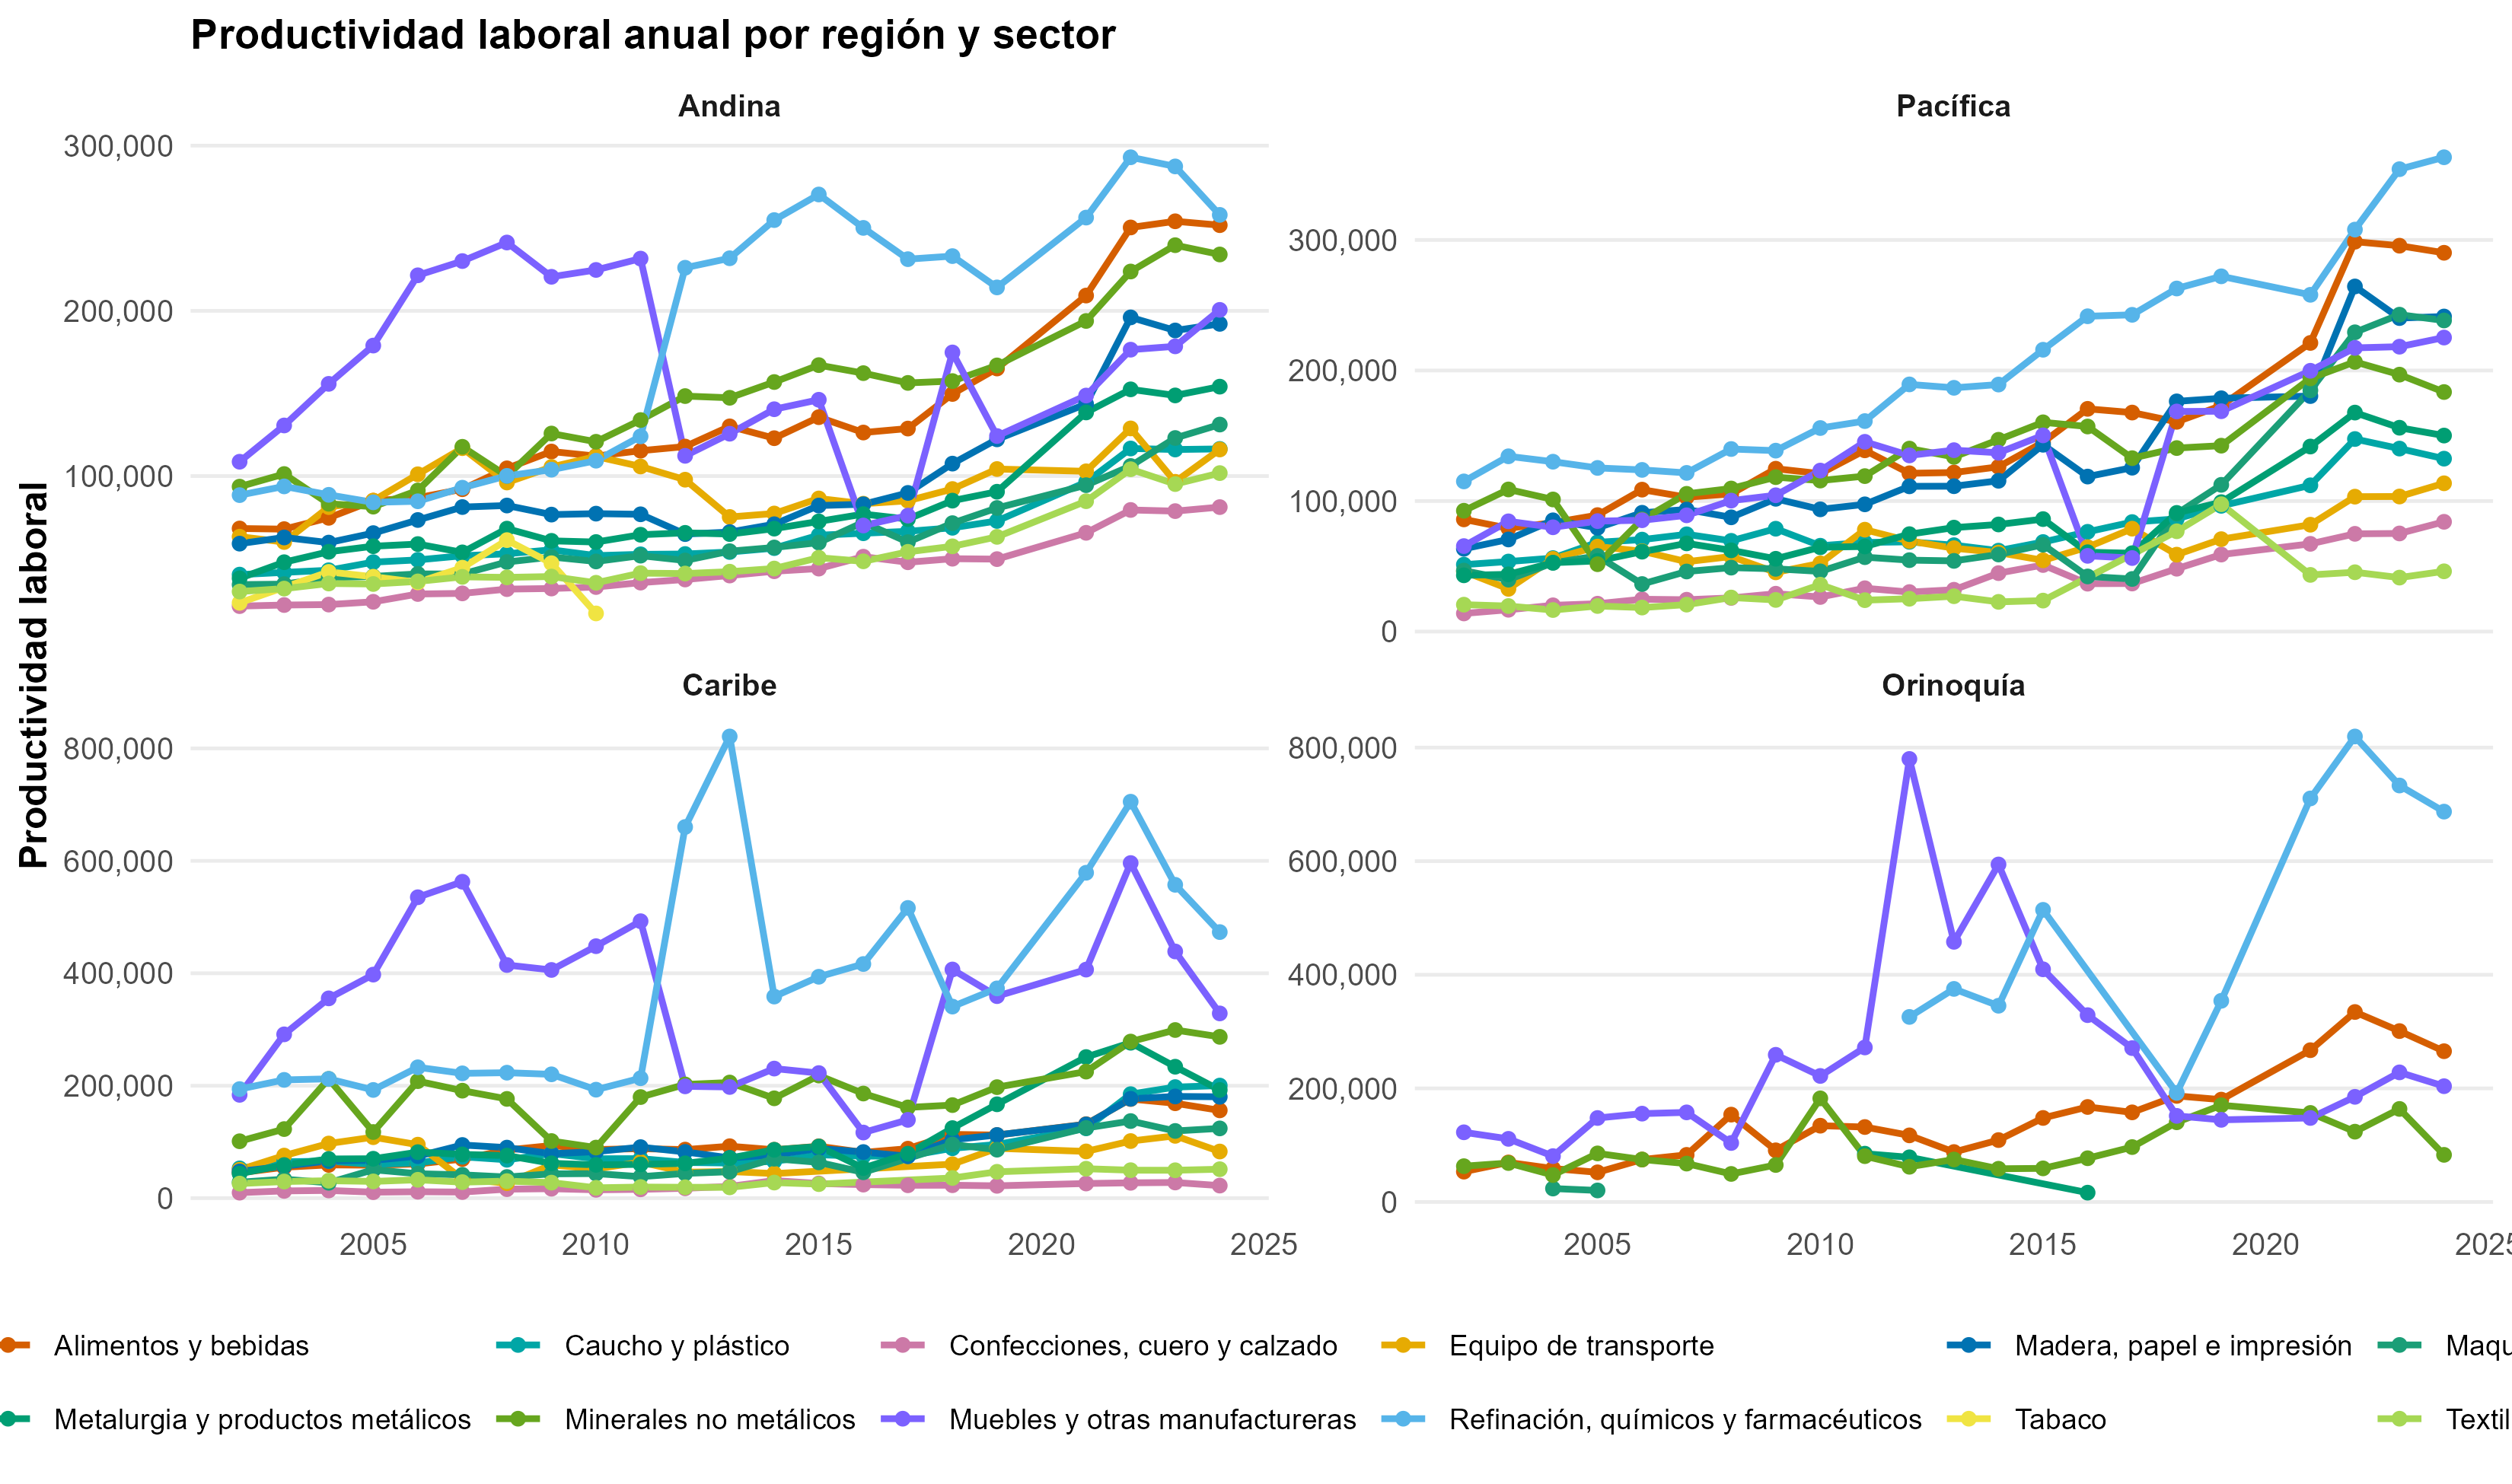
\includegraphics[width=0.9\linewidth]{fig15.png}
\end{frame}

\begin{frame}{Tablas generadas}
  \small
  \begin{itemize}
    \item \texttt{tabla\_total\_anual.csv} y \texttt{tabla\_total\_anual.xlsx}
    \item \texttt{tabla\_sector\_anual.csv} y \texttt{tabla\_sector\_anual.xlsx}
    \item \texttt{EAM\_2024Sectores.xlsx} y \texttt{EAM\_2024Sectores2.xlsx}
    \item \texttt{INGLABO\_ANUAL\_manufactura\_2024.xlsx}
    \item \texttt{INGLABO\_manufactura\_2008.xlsx} a \texttt{INGLABO\_manufactura\_2025.xlsx}
    \item \texttt{Tablas\_Mejoradas\_Sectores\_CON\_FORMULAS.xlsx}
  \end{itemize}
\end{frame}

\begin{frame}{Cierre}
  \begin{itemize}
    \item Mensaje final.
    \item Siguientes pasos.
  \end{itemize}
\end{frame}

\end{document}
